% **************************************************************************************************************
% A Classic Thesis Style
% An Homage to The Elements of Typographic Style
%
% Copyright (C) 2018 André Miede and Ivo Pletikosić
%
% If you like the style then I would appreciate a postcard. My address
% can be found in the file ClassicThesis.pdf. A collection of the
% postcards I received so far is available online at
% http://postcards.miede.de
%
% License:
% This program is free software; you can redistribute it and/or modify
% it under the terms of the GNU General Public License as published by
% the Free Software Foundation; either version 2 of the License, or
% (at your option) any later version.
%
% This program is distributed in the hope that it will be useful,
% but WITHOUT ANY WARRANTY; without even the implied warranty of
% MERCHANTABILITY or FITNESS FOR A PARTICULAR PURPOSE.  See the
% GNU General Public License for more details.
%
% You should have received a copy of the GNU General Public License
% along with this program; see the file COPYING.  If not, write to
% the Free Software Foundation, Inc., 59 Temple Place - Suite 330,
% Boston, MA 02111-1307, USA.
%
% PLEASE SEE ALSO THE AUTHORS' NOTE REGARDING THIS LICENSE
% IN THE DOCUMENTATION (ClassicThesis.pdf --> Chapter 1 / Chapter01.tex)
% **************************************************************************************************************
\RequirePackage{silence} % :-\
    \WarningFilter{scrreprt}{Usage of package `titlesec'}
    %\WarningFilter{scrreprt}{Activating an ugly workaround}
    \WarningFilter{titlesec}{Non standard sectioning command detected}
\documentclass[ twoside,openright,titlepage,numbers=noenddot,%1headlines,
                headinclude,footinclude,cleardoublepage=empty,abstract=on,
                BCOR=5mm,paper=a4,fontsize=11pt
                ]{scrreprt}

%********************************************************************
% Note: Make all your adjustments in here
%*******************************************************
% ****************************************************************************************************
% classicthesis-config.tex
% formerly known as loadpackages.sty, classicthesis-ldpkg.sty, and classicthesis-preamble.sty
% Use it at the beginning of your ClassicThesis.tex, or as a LaTeX Preamble
% in your ClassicThesis.{tex,lyx} with % ****************************************************************************************************
% classicthesis-config.tex
% formerly known as loadpackages.sty, classicthesis-ldpkg.sty, and classicthesis-preamble.sty
% Use it at the beginning of your ClassicThesis.tex, or as a LaTeX Preamble
% in your ClassicThesis.{tex,lyx} with % ****************************************************************************************************
% classicthesis-config.tex
% formerly known as loadpackages.sty, classicthesis-ldpkg.sty, and classicthesis-preamble.sty
% Use it at the beginning of your ClassicThesis.tex, or as a LaTeX Preamble
% in your ClassicThesis.{tex,lyx} with \input{classicthesis-config}
% ****************************************************************************************************
% If you like the classicthesis, then I would appreciate a postcard.
% My address can be found in the file ClassicThesis.pdf. A collection
% of the postcards I received so far is available online at
% http://postcards.miede.de
% ****************************************************************************************************


% ****************************************************************************************************
% 0. Set the encoding of your files. UTF-8 is the only sensible encoding nowadays. If you can't read
% äöüßáéçèê∂åëæƒÏ€ then change the encoding setting in your editor, not the line below. If your editor
% does not support utf8 use another editor!
% ****************************************************************************************************
\PassOptionsToPackage{utf8}{inputenc}
  \usepackage{inputenc}

\PassOptionsToPackage{T1}{fontenc} % T2A for cyrillics
  \usepackage{fontenc}


% ****************************************************************************************************
% 1. Configure classicthesis for your needs here, e.g., remove "drafting" below
% in order to deactivate the time-stamp on the pages
% (see ClassicThesis.pdf for more information):
% ****************************************************************************************************
\PassOptionsToPackage{
  drafting=true,    % print version information on the bottom of the pages
  tocaligned=false, % the left column of the toc will be aligned (no indentation)
  dottedtoc=false,  % page numbers in ToC flushed right
  eulerchapternumbers=true, % use AMS Euler for chapter font (otherwise Palatino)
  linedheaders=false,       % chaper headers will have line above and beneath
  floatperchapter=true,     % numbering per chapter for all floats (i.e., Figure 1.1)
  eulermath=false,  % use awesome Euler fonts for mathematical formulae (only with pdfLaTeX)
  beramono=true,    % toggle a nice monospaced font (w/ bold)
  palatino=true,    % deactivate standard font for loading another one, see the last section at the end of this file for suggestions
  style=classicthesis % classicthesis, arsclassica
}{classicthesis}


% ****************************************************************************************************
% 2. Personal data and user ad-hoc commands (insert your own data here)
% ****************************************************************************************************
\newcommand{\myTitle}{A Classic Thesis Style\xspace}
\newcommand{\mySubtitle}{An Homage to The Elements of Typographic Style\xspace}
\newcommand{\myDegree}{Doktor-Ingenieur (Dr.-Ing.)\xspace}
\newcommand{\myName}{André Miede \& Ivo Pletikosić\xspace}
\newcommand{\myProf}{Put name here\xspace}
\newcommand{\myOtherProf}{Put name here\xspace}
\newcommand{\mySupervisor}{Put name here\xspace}
\newcommand{\myFaculty}{Put data here\xspace}
\newcommand{\myDepartment}{Put data here\xspace}
\newcommand{\myUni}{Put data here\xspace}
\newcommand{\myLocation}{Saarbrücken\xspace}
\newcommand{\myTime}{June 2018\xspace}
\newcommand{\myVersion}{\classicthesis}

% ********************************************************************
% Setup, finetuning, and useful commands
% ********************************************************************
\providecommand{\mLyX}{L\kern-.1667em\lower.25em\hbox{Y}\kern-.125emX\@}
\newcommand{\ie}{i.\,e.}
\newcommand{\Ie}{I.\,e.}
\newcommand{\eg}{e.\,g.}
\newcommand{\Eg}{E.\,g.}
% ****************************************************************************************************


% ****************************************************************************************************
% 3. Loading some handy packages
% ****************************************************************************************************
% ********************************************************************
% Packages with options that might require adjustments
% ********************************************************************
\PassOptionsToPackage{ngerman,american}{babel} % change this to your language(s), main language last
% Spanish languages need extra options in order to work with this template
%\PassOptionsToPackage{spanish,es-lcroman}{babel}
    \usepackage{babel}

\usepackage{csquotes}
\PassOptionsToPackage{%
  %backend=biber,bibencoding=utf8, %instead of bibtex
  backend=bibtex8,bibencoding=ascii,%
  language=auto,%
  style=numeric-comp,%
  %style=authoryear-comp, % Author 1999, 2010
  %bibstyle=authoryear,dashed=false, % dashed: substitute rep. author with ---
  sorting=nyt, % name, year, title
  maxbibnames=10, % default: 3, et al.
  %backref=true,%
  natbib=true % natbib compatibility mode (\citep and \citet still work)
}{biblatex}
    \usepackage{biblatex}

\PassOptionsToPackage{fleqn}{amsmath}       % math environments and more by the AMS
  \usepackage{amsmath}

% ********************************************************************
% General useful packages
% ********************************************************************
\usepackage{graphicx} %
\usepackage{scrhack} % fix warnings when using KOMA with listings package
\usepackage{xspace} % to get the spacing after macros right
\PassOptionsToPackage{printonlyused,smaller}{acronym}
  \usepackage{acronym} % nice macros for handling all acronyms in the thesis
  %\renewcommand{\bflabel}[1]{{#1}\hfill} % fix the list of acronyms --> no longer working
  %\renewcommand*{\acsfont}[1]{\textsc{#1}}
  %\renewcommand*{\aclabelfont}[1]{\acsfont{#1}}
  %\def\bflabel#1{{#1\hfill}}
  \def\bflabel#1{{\acsfont{#1}\hfill}}
  \def\aclabelfont#1{\acsfont{#1}}
% ****************************************************************************************************
%\usepackage{pgfplots} % External TikZ/PGF support (thanks to Andreas Nautsch)
%\usetikzlibrary{external}
%\tikzexternalize[mode=list and make, prefix=ext-tikz/]
% ****************************************************************************************************


% ****************************************************************************************************
% 4. Setup floats: tables, (sub)figures, and captions
% ****************************************************************************************************
\usepackage{tabularx} % better tables
  \setlength{\extrarowheight}{3pt} % increase table row height
\newcommand{\tableheadline}[1]{\multicolumn{1}{l}{\spacedlowsmallcaps{#1}}}
\newcommand{\myfloatalign}{\centering} % to be used with each float for alignment
\usepackage{subfig}
% ****************************************************************************************************


% ****************************************************************************************************
% 5. Setup code listings
% ****************************************************************************************************
\usepackage{listings}
%\lstset{emph={trueIndex,root},emphstyle=\color{BlueViolet}}%\underbar} % for special keywords
\lstset{language=[LaTeX]Tex,%C++,
  morekeywords={PassOptionsToPackage,selectlanguage},
  keywordstyle=\color{RoyalBlue},%\bfseries,
  basicstyle=\small\ttfamily,
  %identifierstyle=\color{NavyBlue},
  commentstyle=\color{Green}\ttfamily,
  stringstyle=\rmfamily,
  numbers=none,%left,%
  numberstyle=\scriptsize,%\tiny
  stepnumber=5,
  numbersep=8pt,
  showstringspaces=false,
  breaklines=true,
  %frameround=ftff,
  %frame=single,
  belowcaptionskip=.75\baselineskip
  %frame=L
}
% ****************************************************************************************************




% ****************************************************************************************************
% 6. Last calls before the bar closes
% ****************************************************************************************************
% ********************************************************************
% Her Majesty herself
% ********************************************************************
\usepackage{classicthesis}


% ********************************************************************
% Fine-tune hyperreferences (hyperref should be called last)
% ********************************************************************
\hypersetup{%
  %draft, % hyperref's draft mode, for printing see below
  colorlinks=true, linktocpage=true, pdfstartpage=3, pdfstartview=FitV,%
  % uncomment the following line if you want to have black links (e.g., for printing)
  %colorlinks=false, linktocpage=false, pdfstartpage=3, pdfstartview=FitV, pdfborder={0 0 0},%
  breaklinks=true, pageanchor=true,%
  pdfpagemode=UseNone, %
  % pdfpagemode=UseOutlines,%
  plainpages=false, bookmarksnumbered, bookmarksopen=true, bookmarksopenlevel=1,%
  hypertexnames=true, pdfhighlight=/O,%nesting=true,%frenchlinks,%
  urlcolor=CTurl, linkcolor=CTlink, citecolor=CTcitation, %pagecolor=RoyalBlue,%
  %urlcolor=Black, linkcolor=Black, citecolor=Black, %pagecolor=Black,%
  pdftitle={\myTitle},%
  pdfauthor={\textcopyright\ \myName, \myUni, \myFaculty},%
  pdfsubject={},%
  pdfkeywords={},%
  pdfcreator={pdfLaTeX},%
  pdfproducer={LaTeX with hyperref and classicthesis}%
}


% ********************************************************************
% Setup autoreferences (hyperref and babel)
% ********************************************************************
% There are some issues regarding autorefnames
% http://www.tex.ac.uk/cgi-bin/texfaq2html?label=latexwords
% you have to redefine the macros for the
% language you use, e.g., american, ngerman
% (as chosen when loading babel/AtBeginDocument)
% ********************************************************************
\makeatletter
\@ifpackageloaded{babel}%
  {%
    \addto\extrasamerican{%
      \renewcommand*{\figureautorefname}{Figure}%
      \renewcommand*{\tableautorefname}{Table}%
      \renewcommand*{\partautorefname}{Part}%
      \renewcommand*{\chapterautorefname}{Chapter}%
      \renewcommand*{\sectionautorefname}{Section}%
      \renewcommand*{\subsectionautorefname}{Section}%
      \renewcommand*{\subsubsectionautorefname}{Section}%
    }%
    \addto\extrasngerman{%
      \renewcommand*{\paragraphautorefname}{Absatz}%
      \renewcommand*{\subparagraphautorefname}{Unterabsatz}%
      \renewcommand*{\footnoteautorefname}{Fu\"snote}%
      \renewcommand*{\FancyVerbLineautorefname}{Zeile}%
      \renewcommand*{\theoremautorefname}{Theorem}%
      \renewcommand*{\appendixautorefname}{Anhang}%
      \renewcommand*{\equationautorefname}{Gleichung}%
      \renewcommand*{\itemautorefname}{Punkt}%
    }%
      % Fix to getting autorefs for subfigures right (thanks to Belinda Vogt for changing the definition)
      \providecommand{\subfigureautorefname}{\figureautorefname}%
    }{\relax}
\makeatother


% ********************************************************************
% Development Stuff
% ********************************************************************
\listfiles
%\PassOptionsToPackage{l2tabu,orthodox,abort}{nag}
%  \usepackage{nag}
%\PassOptionsToPackage{warning, all}{onlyamsmath}
%  \usepackage{onlyamsmath}


% ****************************************************************************************************
% 7. Further adjustments (experimental)
% ****************************************************************************************************
% ********************************************************************
% Changing the text area
% ********************************************************************
%\areaset[current]{312pt}{761pt} % 686 (factor 2.2) + 33 head + 42 head \the\footskip
%\setlength{\marginparwidth}{7em}%
%\setlength{\marginparsep}{2em}%

% ********************************************************************
% Using different fonts
% ********************************************************************
%\usepackage[oldstylenums]{kpfonts} % oldstyle notextcomp
% \usepackage[osf]{libertine}
%\usepackage[light,condensed,math]{iwona}
%\renewcommand{\sfdefault}{iwona}
%\usepackage{lmodern} % <-- no osf support :-(
%\usepackage{cfr-lm} %
%\usepackage[urw-garamond]{mathdesign} <-- no osf support :-(
%\usepackage[default,osfigures]{opensans} % scale=0.95
%\usepackage[sfdefault]{FiraSans}
% \usepackage[opticals,mathlf]{MinionPro} % onlytext
% ********************************************************************
%\usepackage[largesc,osf]{newpxtext}
%\linespread{1.05} % a bit more for Palatino
% Used to fix these:
% https://bitbucket.org/amiede/classicthesis/issues/139/italics-in-pallatino-capitals-chapter
% https://bitbucket.org/amiede/classicthesis/issues/45/problema-testatine-su-classicthesis-style
% ********************************************************************
% ****************************************************************************************************

% ****************************************************************************************************
% If you like the classicthesis, then I would appreciate a postcard.
% My address can be found in the file ClassicThesis.pdf. A collection
% of the postcards I received so far is available online at
% http://postcards.miede.de
% ****************************************************************************************************


% ****************************************************************************************************
% 0. Set the encoding of your files. UTF-8 is the only sensible encoding nowadays. If you can't read
% äöüßáéçèê∂åëæƒÏ€ then change the encoding setting in your editor, not the line below. If your editor
% does not support utf8 use another editor!
% ****************************************************************************************************
\PassOptionsToPackage{utf8}{inputenc}
  \usepackage{inputenc}

\PassOptionsToPackage{T1}{fontenc} % T2A for cyrillics
  \usepackage{fontenc}


% ****************************************************************************************************
% 1. Configure classicthesis for your needs here, e.g., remove "drafting" below
% in order to deactivate the time-stamp on the pages
% (see ClassicThesis.pdf for more information):
% ****************************************************************************************************
\PassOptionsToPackage{
  drafting=true,    % print version information on the bottom of the pages
  tocaligned=false, % the left column of the toc will be aligned (no indentation)
  dottedtoc=false,  % page numbers in ToC flushed right
  eulerchapternumbers=true, % use AMS Euler for chapter font (otherwise Palatino)
  linedheaders=false,       % chaper headers will have line above and beneath
  floatperchapter=true,     % numbering per chapter for all floats (i.e., Figure 1.1)
  eulermath=false,  % use awesome Euler fonts for mathematical formulae (only with pdfLaTeX)
  beramono=true,    % toggle a nice monospaced font (w/ bold)
  palatino=true,    % deactivate standard font for loading another one, see the last section at the end of this file for suggestions
  style=classicthesis % classicthesis, arsclassica
}{classicthesis}


% ****************************************************************************************************
% 2. Personal data and user ad-hoc commands (insert your own data here)
% ****************************************************************************************************
\newcommand{\myTitle}{A Classic Thesis Style\xspace}
\newcommand{\mySubtitle}{An Homage to The Elements of Typographic Style\xspace}
\newcommand{\myDegree}{Doktor-Ingenieur (Dr.-Ing.)\xspace}
\newcommand{\myName}{André Miede \& Ivo Pletikosić\xspace}
\newcommand{\myProf}{Put name here\xspace}
\newcommand{\myOtherProf}{Put name here\xspace}
\newcommand{\mySupervisor}{Put name here\xspace}
\newcommand{\myFaculty}{Put data here\xspace}
\newcommand{\myDepartment}{Put data here\xspace}
\newcommand{\myUni}{Put data here\xspace}
\newcommand{\myLocation}{Saarbrücken\xspace}
\newcommand{\myTime}{June 2018\xspace}
\newcommand{\myVersion}{\classicthesis}

% ********************************************************************
% Setup, finetuning, and useful commands
% ********************************************************************
\providecommand{\mLyX}{L\kern-.1667em\lower.25em\hbox{Y}\kern-.125emX\@}
\newcommand{\ie}{i.\,e.}
\newcommand{\Ie}{I.\,e.}
\newcommand{\eg}{e.\,g.}
\newcommand{\Eg}{E.\,g.}
% ****************************************************************************************************


% ****************************************************************************************************
% 3. Loading some handy packages
% ****************************************************************************************************
% ********************************************************************
% Packages with options that might require adjustments
% ********************************************************************
\PassOptionsToPackage{ngerman,american}{babel} % change this to your language(s), main language last
% Spanish languages need extra options in order to work with this template
%\PassOptionsToPackage{spanish,es-lcroman}{babel}
    \usepackage{babel}

\usepackage{csquotes}
\PassOptionsToPackage{%
  %backend=biber,bibencoding=utf8, %instead of bibtex
  backend=bibtex8,bibencoding=ascii,%
  language=auto,%
  style=numeric-comp,%
  %style=authoryear-comp, % Author 1999, 2010
  %bibstyle=authoryear,dashed=false, % dashed: substitute rep. author with ---
  sorting=nyt, % name, year, title
  maxbibnames=10, % default: 3, et al.
  %backref=true,%
  natbib=true % natbib compatibility mode (\citep and \citet still work)
}{biblatex}
    \usepackage{biblatex}

\PassOptionsToPackage{fleqn}{amsmath}       % math environments and more by the AMS
  \usepackage{amsmath}

% ********************************************************************
% General useful packages
% ********************************************************************
\usepackage{graphicx} %
\usepackage{scrhack} % fix warnings when using KOMA with listings package
\usepackage{xspace} % to get the spacing after macros right
\PassOptionsToPackage{printonlyused,smaller}{acronym}
  \usepackage{acronym} % nice macros for handling all acronyms in the thesis
  %\renewcommand{\bflabel}[1]{{#1}\hfill} % fix the list of acronyms --> no longer working
  %\renewcommand*{\acsfont}[1]{\textsc{#1}}
  %\renewcommand*{\aclabelfont}[1]{\acsfont{#1}}
  %\def\bflabel#1{{#1\hfill}}
  \def\bflabel#1{{\acsfont{#1}\hfill}}
  \def\aclabelfont#1{\acsfont{#1}}
% ****************************************************************************************************
%\usepackage{pgfplots} % External TikZ/PGF support (thanks to Andreas Nautsch)
%\usetikzlibrary{external}
%\tikzexternalize[mode=list and make, prefix=ext-tikz/]
% ****************************************************************************************************


% ****************************************************************************************************
% 4. Setup floats: tables, (sub)figures, and captions
% ****************************************************************************************************
\usepackage{tabularx} % better tables
  \setlength{\extrarowheight}{3pt} % increase table row height
\newcommand{\tableheadline}[1]{\multicolumn{1}{l}{\spacedlowsmallcaps{#1}}}
\newcommand{\myfloatalign}{\centering} % to be used with each float for alignment
\usepackage{subfig}
% ****************************************************************************************************


% ****************************************************************************************************
% 5. Setup code listings
% ****************************************************************************************************
\usepackage{listings}
%\lstset{emph={trueIndex,root},emphstyle=\color{BlueViolet}}%\underbar} % for special keywords
\lstset{language=[LaTeX]Tex,%C++,
  morekeywords={PassOptionsToPackage,selectlanguage},
  keywordstyle=\color{RoyalBlue},%\bfseries,
  basicstyle=\small\ttfamily,
  %identifierstyle=\color{NavyBlue},
  commentstyle=\color{Green}\ttfamily,
  stringstyle=\rmfamily,
  numbers=none,%left,%
  numberstyle=\scriptsize,%\tiny
  stepnumber=5,
  numbersep=8pt,
  showstringspaces=false,
  breaklines=true,
  %frameround=ftff,
  %frame=single,
  belowcaptionskip=.75\baselineskip
  %frame=L
}
% ****************************************************************************************************




% ****************************************************************************************************
% 6. Last calls before the bar closes
% ****************************************************************************************************
% ********************************************************************
% Her Majesty herself
% ********************************************************************
\usepackage{classicthesis}


% ********************************************************************
% Fine-tune hyperreferences (hyperref should be called last)
% ********************************************************************
\hypersetup{%
  %draft, % hyperref's draft mode, for printing see below
  colorlinks=true, linktocpage=true, pdfstartpage=3, pdfstartview=FitV,%
  % uncomment the following line if you want to have black links (e.g., for printing)
  %colorlinks=false, linktocpage=false, pdfstartpage=3, pdfstartview=FitV, pdfborder={0 0 0},%
  breaklinks=true, pageanchor=true,%
  pdfpagemode=UseNone, %
  % pdfpagemode=UseOutlines,%
  plainpages=false, bookmarksnumbered, bookmarksopen=true, bookmarksopenlevel=1,%
  hypertexnames=true, pdfhighlight=/O,%nesting=true,%frenchlinks,%
  urlcolor=CTurl, linkcolor=CTlink, citecolor=CTcitation, %pagecolor=RoyalBlue,%
  %urlcolor=Black, linkcolor=Black, citecolor=Black, %pagecolor=Black,%
  pdftitle={\myTitle},%
  pdfauthor={\textcopyright\ \myName, \myUni, \myFaculty},%
  pdfsubject={},%
  pdfkeywords={},%
  pdfcreator={pdfLaTeX},%
  pdfproducer={LaTeX with hyperref and classicthesis}%
}


% ********************************************************************
% Setup autoreferences (hyperref and babel)
% ********************************************************************
% There are some issues regarding autorefnames
% http://www.tex.ac.uk/cgi-bin/texfaq2html?label=latexwords
% you have to redefine the macros for the
% language you use, e.g., american, ngerman
% (as chosen when loading babel/AtBeginDocument)
% ********************************************************************
\makeatletter
\@ifpackageloaded{babel}%
  {%
    \addto\extrasamerican{%
      \renewcommand*{\figureautorefname}{Figure}%
      \renewcommand*{\tableautorefname}{Table}%
      \renewcommand*{\partautorefname}{Part}%
      \renewcommand*{\chapterautorefname}{Chapter}%
      \renewcommand*{\sectionautorefname}{Section}%
      \renewcommand*{\subsectionautorefname}{Section}%
      \renewcommand*{\subsubsectionautorefname}{Section}%
    }%
    \addto\extrasngerman{%
      \renewcommand*{\paragraphautorefname}{Absatz}%
      \renewcommand*{\subparagraphautorefname}{Unterabsatz}%
      \renewcommand*{\footnoteautorefname}{Fu\"snote}%
      \renewcommand*{\FancyVerbLineautorefname}{Zeile}%
      \renewcommand*{\theoremautorefname}{Theorem}%
      \renewcommand*{\appendixautorefname}{Anhang}%
      \renewcommand*{\equationautorefname}{Gleichung}%
      \renewcommand*{\itemautorefname}{Punkt}%
    }%
      % Fix to getting autorefs for subfigures right (thanks to Belinda Vogt for changing the definition)
      \providecommand{\subfigureautorefname}{\figureautorefname}%
    }{\relax}
\makeatother


% ********************************************************************
% Development Stuff
% ********************************************************************
\listfiles
%\PassOptionsToPackage{l2tabu,orthodox,abort}{nag}
%  \usepackage{nag}
%\PassOptionsToPackage{warning, all}{onlyamsmath}
%  \usepackage{onlyamsmath}


% ****************************************************************************************************
% 7. Further adjustments (experimental)
% ****************************************************************************************************
% ********************************************************************
% Changing the text area
% ********************************************************************
%\areaset[current]{312pt}{761pt} % 686 (factor 2.2) + 33 head + 42 head \the\footskip
%\setlength{\marginparwidth}{7em}%
%\setlength{\marginparsep}{2em}%

% ********************************************************************
% Using different fonts
% ********************************************************************
%\usepackage[oldstylenums]{kpfonts} % oldstyle notextcomp
% \usepackage[osf]{libertine}
%\usepackage[light,condensed,math]{iwona}
%\renewcommand{\sfdefault}{iwona}
%\usepackage{lmodern} % <-- no osf support :-(
%\usepackage{cfr-lm} %
%\usepackage[urw-garamond]{mathdesign} <-- no osf support :-(
%\usepackage[default,osfigures]{opensans} % scale=0.95
%\usepackage[sfdefault]{FiraSans}
% \usepackage[opticals,mathlf]{MinionPro} % onlytext
% ********************************************************************
%\usepackage[largesc,osf]{newpxtext}
%\linespread{1.05} % a bit more for Palatino
% Used to fix these:
% https://bitbucket.org/amiede/classicthesis/issues/139/italics-in-pallatino-capitals-chapter
% https://bitbucket.org/amiede/classicthesis/issues/45/problema-testatine-su-classicthesis-style
% ********************************************************************
% ****************************************************************************************************

% ****************************************************************************************************
% If you like the classicthesis, then I would appreciate a postcard.
% My address can be found in the file ClassicThesis.pdf. A collection
% of the postcards I received so far is available online at
% http://postcards.miede.de
% ****************************************************************************************************


% ****************************************************************************************************
% 0. Set the encoding of your files. UTF-8 is the only sensible encoding nowadays. If you can't read
% äöüßáéçèê∂åëæƒÏ€ then change the encoding setting in your editor, not the line below. If your editor
% does not support utf8 use another editor!
% ****************************************************************************************************
\PassOptionsToPackage{utf8}{inputenc}
  \usepackage{inputenc}

\PassOptionsToPackage{T1}{fontenc} % T2A for cyrillics
  \usepackage{fontenc}


% ****************************************************************************************************
% 1. Configure classicthesis for your needs here, e.g., remove "drafting" below
% in order to deactivate the time-stamp on the pages
% (see ClassicThesis.pdf for more information):
% ****************************************************************************************************
\PassOptionsToPackage{
  drafting=true,    % print version information on the bottom of the pages
  tocaligned=false, % the left column of the toc will be aligned (no indentation)
  dottedtoc=false,  % page numbers in ToC flushed right
  eulerchapternumbers=true, % use AMS Euler for chapter font (otherwise Palatino)
  linedheaders=false,       % chaper headers will have line above and beneath
  floatperchapter=true,     % numbering per chapter for all floats (i.e., Figure 1.1)
  eulermath=false,  % use awesome Euler fonts for mathematical formulae (only with pdfLaTeX)
  beramono=true,    % toggle a nice monospaced font (w/ bold)
  palatino=true,    % deactivate standard font for loading another one, see the last section at the end of this file for suggestions
  style=classicthesis % classicthesis, arsclassica
}{classicthesis}


% ****************************************************************************************************
% 2. Personal data and user ad-hoc commands (insert your own data here)
% ****************************************************************************************************
\newcommand{\myTitle}{A Classic Thesis Style\xspace}
\newcommand{\mySubtitle}{An Homage to The Elements of Typographic Style\xspace}
\newcommand{\myDegree}{Doktor-Ingenieur (Dr.-Ing.)\xspace}
\newcommand{\myName}{André Miede \& Ivo Pletikosić\xspace}
\newcommand{\myProf}{Put name here\xspace}
\newcommand{\myOtherProf}{Put name here\xspace}
\newcommand{\mySupervisor}{Put name here\xspace}
\newcommand{\myFaculty}{Put data here\xspace}
\newcommand{\myDepartment}{Put data here\xspace}
\newcommand{\myUni}{Put data here\xspace}
\newcommand{\myLocation}{Saarbrücken\xspace}
\newcommand{\myTime}{June 2018\xspace}
\newcommand{\myVersion}{\classicthesis}

% ********************************************************************
% Setup, finetuning, and useful commands
% ********************************************************************
\providecommand{\mLyX}{L\kern-.1667em\lower.25em\hbox{Y}\kern-.125emX\@}
\newcommand{\ie}{i.\,e.}
\newcommand{\Ie}{I.\,e.}
\newcommand{\eg}{e.\,g.}
\newcommand{\Eg}{E.\,g.}
% ****************************************************************************************************


% ****************************************************************************************************
% 3. Loading some handy packages
% ****************************************************************************************************
% ********************************************************************
% Packages with options that might require adjustments
% ********************************************************************
\PassOptionsToPackage{ngerman,american}{babel} % change this to your language(s), main language last
% Spanish languages need extra options in order to work with this template
%\PassOptionsToPackage{spanish,es-lcroman}{babel}
    \usepackage{babel}

\usepackage{csquotes}
\PassOptionsToPackage{%
  %backend=biber,bibencoding=utf8, %instead of bibtex
  backend=bibtex8,bibencoding=ascii,%
  language=auto,%
  style=numeric-comp,%
  %style=authoryear-comp, % Author 1999, 2010
  %bibstyle=authoryear,dashed=false, % dashed: substitute rep. author with ---
  sorting=nyt, % name, year, title
  maxbibnames=10, % default: 3, et al.
  %backref=true,%
  natbib=true % natbib compatibility mode (\citep and \citet still work)
}{biblatex}
    \usepackage{biblatex}

\PassOptionsToPackage{fleqn}{amsmath}       % math environments and more by the AMS
  \usepackage{amsmath}

% ********************************************************************
% General useful packages
% ********************************************************************
\usepackage{graphicx} %
\usepackage{scrhack} % fix warnings when using KOMA with listings package
\usepackage{xspace} % to get the spacing after macros right
\PassOptionsToPackage{printonlyused,smaller}{acronym}
  \usepackage{acronym} % nice macros for handling all acronyms in the thesis
  %\renewcommand{\bflabel}[1]{{#1}\hfill} % fix the list of acronyms --> no longer working
  %\renewcommand*{\acsfont}[1]{\textsc{#1}}
  %\renewcommand*{\aclabelfont}[1]{\acsfont{#1}}
  %\def\bflabel#1{{#1\hfill}}
  \def\bflabel#1{{\acsfont{#1}\hfill}}
  \def\aclabelfont#1{\acsfont{#1}}
% ****************************************************************************************************
%\usepackage{pgfplots} % External TikZ/PGF support (thanks to Andreas Nautsch)
%\usetikzlibrary{external}
%\tikzexternalize[mode=list and make, prefix=ext-tikz/]
% ****************************************************************************************************


% ****************************************************************************************************
% 4. Setup floats: tables, (sub)figures, and captions
% ****************************************************************************************************
\usepackage{tabularx} % better tables
  \setlength{\extrarowheight}{3pt} % increase table row height
\newcommand{\tableheadline}[1]{\multicolumn{1}{l}{\spacedlowsmallcaps{#1}}}
\newcommand{\myfloatalign}{\centering} % to be used with each float for alignment
\usepackage{subfig}
% ****************************************************************************************************


% ****************************************************************************************************
% 5. Setup code listings
% ****************************************************************************************************
\usepackage{listings}
%\lstset{emph={trueIndex,root},emphstyle=\color{BlueViolet}}%\underbar} % for special keywords
\lstset{language=[LaTeX]Tex,%C++,
  morekeywords={PassOptionsToPackage,selectlanguage},
  keywordstyle=\color{RoyalBlue},%\bfseries,
  basicstyle=\small\ttfamily,
  %identifierstyle=\color{NavyBlue},
  commentstyle=\color{Green}\ttfamily,
  stringstyle=\rmfamily,
  numbers=none,%left,%
  numberstyle=\scriptsize,%\tiny
  stepnumber=5,
  numbersep=8pt,
  showstringspaces=false,
  breaklines=true,
  %frameround=ftff,
  %frame=single,
  belowcaptionskip=.75\baselineskip
  %frame=L
}
% ****************************************************************************************************




% ****************************************************************************************************
% 6. Last calls before the bar closes
% ****************************************************************************************************
% ********************************************************************
% Her Majesty herself
% ********************************************************************
\usepackage{classicthesis}


% ********************************************************************
% Fine-tune hyperreferences (hyperref should be called last)
% ********************************************************************
\hypersetup{%
  %draft, % hyperref's draft mode, for printing see below
  colorlinks=true, linktocpage=true, pdfstartpage=3, pdfstartview=FitV,%
  % uncomment the following line if you want to have black links (e.g., for printing)
  %colorlinks=false, linktocpage=false, pdfstartpage=3, pdfstartview=FitV, pdfborder={0 0 0},%
  breaklinks=true, pageanchor=true,%
  pdfpagemode=UseNone, %
  % pdfpagemode=UseOutlines,%
  plainpages=false, bookmarksnumbered, bookmarksopen=true, bookmarksopenlevel=1,%
  hypertexnames=true, pdfhighlight=/O,%nesting=true,%frenchlinks,%
  urlcolor=CTurl, linkcolor=CTlink, citecolor=CTcitation, %pagecolor=RoyalBlue,%
  %urlcolor=Black, linkcolor=Black, citecolor=Black, %pagecolor=Black,%
  pdftitle={\myTitle},%
  pdfauthor={\textcopyright\ \myName, \myUni, \myFaculty},%
  pdfsubject={},%
  pdfkeywords={},%
  pdfcreator={pdfLaTeX},%
  pdfproducer={LaTeX with hyperref and classicthesis}%
}


% ********************************************************************
% Setup autoreferences (hyperref and babel)
% ********************************************************************
% There are some issues regarding autorefnames
% http://www.tex.ac.uk/cgi-bin/texfaq2html?label=latexwords
% you have to redefine the macros for the
% language you use, e.g., american, ngerman
% (as chosen when loading babel/AtBeginDocument)
% ********************************************************************
\makeatletter
\@ifpackageloaded{babel}%
  {%
    \addto\extrasamerican{%
      \renewcommand*{\figureautorefname}{Figure}%
      \renewcommand*{\tableautorefname}{Table}%
      \renewcommand*{\partautorefname}{Part}%
      \renewcommand*{\chapterautorefname}{Chapter}%
      \renewcommand*{\sectionautorefname}{Section}%
      \renewcommand*{\subsectionautorefname}{Section}%
      \renewcommand*{\subsubsectionautorefname}{Section}%
    }%
    \addto\extrasngerman{%
      \renewcommand*{\paragraphautorefname}{Absatz}%
      \renewcommand*{\subparagraphautorefname}{Unterabsatz}%
      \renewcommand*{\footnoteautorefname}{Fu\"snote}%
      \renewcommand*{\FancyVerbLineautorefname}{Zeile}%
      \renewcommand*{\theoremautorefname}{Theorem}%
      \renewcommand*{\appendixautorefname}{Anhang}%
      \renewcommand*{\equationautorefname}{Gleichung}%
      \renewcommand*{\itemautorefname}{Punkt}%
    }%
      % Fix to getting autorefs for subfigures right (thanks to Belinda Vogt for changing the definition)
      \providecommand{\subfigureautorefname}{\figureautorefname}%
    }{\relax}
\makeatother


% ********************************************************************
% Development Stuff
% ********************************************************************
\listfiles
%\PassOptionsToPackage{l2tabu,orthodox,abort}{nag}
%  \usepackage{nag}
%\PassOptionsToPackage{warning, all}{onlyamsmath}
%  \usepackage{onlyamsmath}


% ****************************************************************************************************
% 7. Further adjustments (experimental)
% ****************************************************************************************************
% ********************************************************************
% Changing the text area
% ********************************************************************
%\areaset[current]{312pt}{761pt} % 686 (factor 2.2) + 33 head + 42 head \the\footskip
%\setlength{\marginparwidth}{7em}%
%\setlength{\marginparsep}{2em}%

% ********************************************************************
% Using different fonts
% ********************************************************************
%\usepackage[oldstylenums]{kpfonts} % oldstyle notextcomp
% \usepackage[osf]{libertine}
%\usepackage[light,condensed,math]{iwona}
%\renewcommand{\sfdefault}{iwona}
%\usepackage{lmodern} % <-- no osf support :-(
%\usepackage{cfr-lm} %
%\usepackage[urw-garamond]{mathdesign} <-- no osf support :-(
%\usepackage[default,osfigures]{opensans} % scale=0.95
%\usepackage[sfdefault]{FiraSans}
% \usepackage[opticals,mathlf]{MinionPro} % onlytext
% ********************************************************************
%\usepackage[largesc,osf]{newpxtext}
%\linespread{1.05} % a bit more for Palatino
% Used to fix these:
% https://bitbucket.org/amiede/classicthesis/issues/139/italics-in-pallatino-capitals-chapter
% https://bitbucket.org/amiede/classicthesis/issues/45/problema-testatine-su-classicthesis-style
% ********************************************************************
% ****************************************************************************************************


%********************************************************************
% Bibliographies
%*******************************************************
\addbibresource{Bibliography.bib}
\addbibresource[label=ownpubs]{AMiede_Publications.bib}

%********************************************************************
% Hyphenation
%*******************************************************
%\hyphenation{put special hyphenation here}

% ********************************************************************
% GO!GO!GO! MOVE IT!
%*******************************************************
\begin{document}
\frenchspacing
\raggedbottom
\selectlanguage{american} % american ngerman
%\renewcommand*{\bibname}{new name}
%\setbibpreamble{}
\pagenumbering{roman}
\pagestyle{plain}
%********************************************************************
% Frontmatter
%*******************************************************
%*******************************************************
% Little Dirty Titlepage
%*******************************************************
\thispagestyle{empty}
%\pdfbookmark[1]{Titel}{title}
%*******************************************************
\begin{center}
    \spacedlowsmallcaps{\myName} \\ \medskip

    \begingroup
        \color{CTtitle}\spacedallcaps{\myTitle}
    \endgroup
\end{center}

%*******************************************************
% Titlepage
%*******************************************************
\begin{titlepage}
    %\pdfbookmark[1]{\myTitle}{titlepage}
    % if you want the titlepage to be centered, uncomment and fine-tune the line below (KOMA classes environment)
    \begin{addmargin}[-1cm]{-3cm}
    \begin{center}
        \large

        \hfill

        \vfill

        \begingroup
            \color{CTtitle}\spacedallcaps{\myTitle} \\ \bigskip
        \endgroup

        \spacedlowsmallcaps{\myName}

        \vfill

        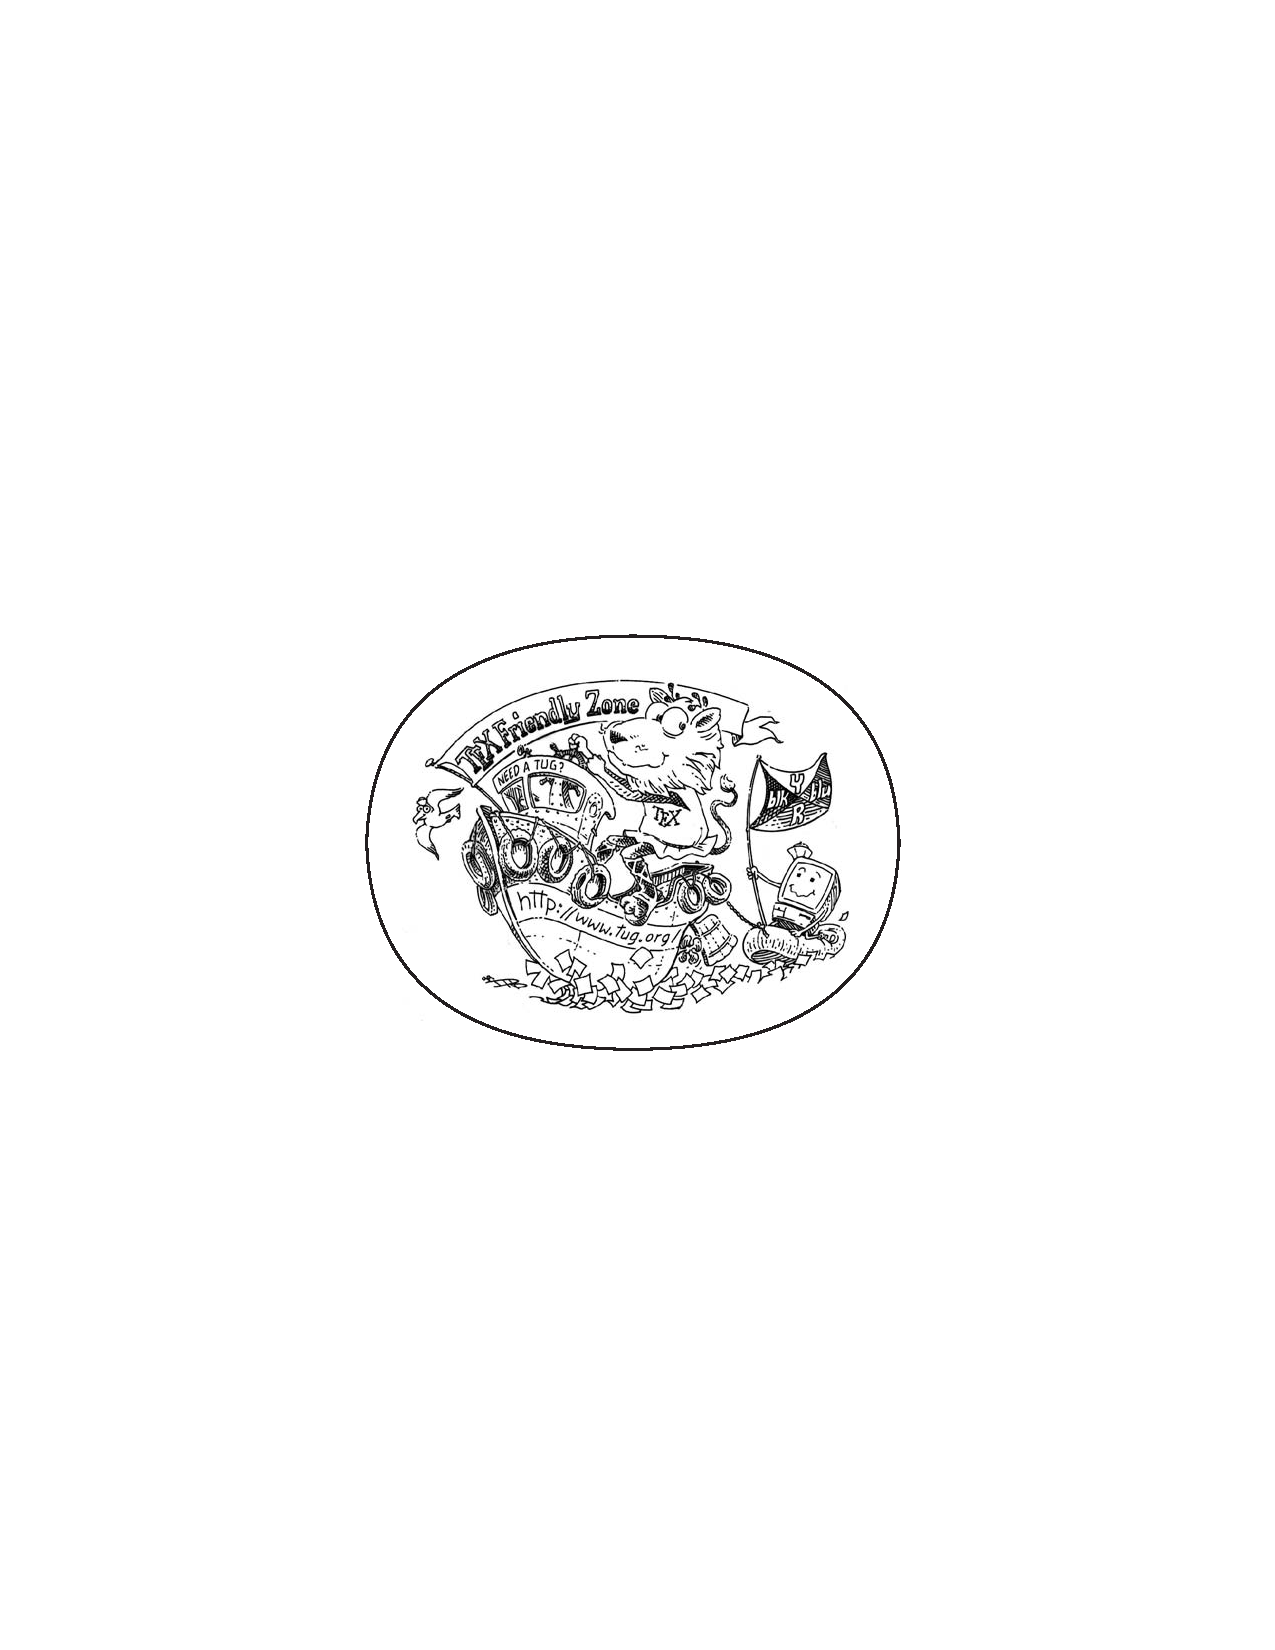
\includegraphics[width=6cm]{gfx/TFZsuperellipse_bw} \\ \medskip

        \mySubtitle \\ \medskip
        %\myDegree \\
        %\myDepartment \\
        %\myFaculty \\
        %\myUni \\ \bigskip

        \myTime\ -- \myVersion

        \vfill

    \end{center}
  \end{addmargin}
\end{titlepage}

\thispagestyle{empty}

\hfill

\vfill

\noindent\myName: \textit{\myTitle,} \mySubtitle, %\myDegree,
\textcopyright\ \myTime

%\bigskip
%
%\noindent\spacedlowsmallcaps{Supervisors}: \\
%\myProf \\
%\myOtherProf \\
%\mySupervisor
%
%\medskip
%
%\noindent\spacedlowsmallcaps{Location}: \\
%\myLocation
%
%\medskip
%
%\noindent\spacedlowsmallcaps{Time Frame}: \\
%\myTime

\cleardoublepage%*******************************************************
% Dedication
%*******************************************************
\thispagestyle{empty}
\phantomsection
\pdfbookmark[1]{Dedication}{Dedication}

\vspace*{3cm}

\begin{center}
    \emph{Ohana} means family. \\
    Family means nobody gets left behind, or forgotten. \\ \medskip
    --- Lilo \& Stitch
\end{center}

\medskip

\begin{center}
    Dedicated to the loving memory of Rudolf Miede. \\ \smallskip
    1939\,--\,2005
\end{center}

%\cleardoublepage\include{FrontBackmatter/Foreword}
\cleardoublepage%*******************************************************
% Abstract
%*******************************************************
%\renewcommand{\abstractname}{Abstract}
\pdfbookmark[1]{Abstract}{Abstract}
% \addcontentsline{toc}{chapter}{\tocEntry{Abstract}}
\begingroup
\let\clearpage\relax
\let\cleardoublepage\relax
\let\cleardoublepage\relax

\chapter*{Abstract}
Short summary of the contents in English\dots a great guide by
Kent Beck how to write good abstracts can be found here:
\begin{center}
\url{https://plg.uwaterloo.ca/~migod/research/beckOOPSLA.html}
\end{center}

\vfill

\begin{otherlanguage}{ngerman}
\pdfbookmark[1]{Zusammenfassung}{Zusammenfassung}
\chapter*{Zusammenfassung}
Kurze Zusammenfassung des Inhaltes in deutscher Sprache\dots
\end{otherlanguage}

\endgroup

\vfill

\cleardoublepage%*******************************************************
% Publications
%*******************************************************
\pdfbookmark[1]{Publications}{publications}
\chapter*{Publications}\graffito{This is just an early --~and currently ugly~-- test!}
This might come in handy for PhD theses: some ideas and figures have appeared previously in the following publications:

%\noindent Put your publications from the thesis here. The packages \texttt{multibib} or \texttt{bibtopic} etc. can be used to handle multiple different bibliographies in your document.

\begin{refsection}[ownpubs]
    \small
    \nocite{*} % is local to to the enclosing refsection
    \printbibliography[heading=none]
\end{refsection}

\emph{Attention}: This requires a separate run of \texttt{bibtex} for your \texttt{refsection}, \eg, \texttt{ClassicThesis1-blx} for this file. You might also use \texttt{biber} as the backend for \texttt{biblatex}. See also \url{http://tex.stackexchange.com/questions/128196/problem-with-refsection}.

\cleardoublepage%*******************************************************
% Acknowledgments
%*******************************************************
\pdfbookmark[1]{Acknowledgments}{acknowledgments}

\begin{flushright}{\slshape
    "A self-organizing system acts autonomously, as if the interconnecting  \\
    components had a single mind. And as these components spontaneously\\
    march to the beat of their own drummer, they organize, adapt,\\
    and evolve toward a greater complexity than one would ever\\
    expect just by looking at the parts by themselves."} \\ \medskip
    --- \defcitealias{samuels_defense_2013}{L. K. Samuels}\citetalias{samuels_defense_2013} \citep{samuels_defense_2013}
\end{flushright}

\bigskip

\begingroup
\let\clearpage\relax
\let\cleardoublepage\relax
\let\cleardoublepage\relax
\chapter*{Acknowledgments}
   I would like to thank everyone who has graciously provided me with their support and validation through the entire process of writing this thesis. Thank you to Srinivas Gorur-Shandilya, who made all of this possible and encouraged me to pursue this, despite everything. Thank you to Eve Marder who took me in and, without asking, re-arranged my life and education in ways I will forever be grateful for.
   
   I could not have done this without my family, either. Thank you to Sophia, Bobby, Nikki, Miles, Hayden, and Cam. And finally, thank you to my chosen family. Thank you to everyone who has spent countless hours with me talking and philosophizing about science and the world, to everyone who has pushed me to be better than I am now, and most importantly, made the choice to love and support me in ways I will forever remember and be grateful for.

\bigskip

%\noindent\emph{Regarding \mLyX}: The \mLyX\ port was intially done by
%\emph{Nicholas Mariette} in March 2009 and continued by
%\emph{Ivo Pletikosi\'c} in 2011. Thank you very much for your
%work and for the contributions to the original style.


\endgroup

\cleardoublepage%*******************************************************
% Table of Contents
%*******************************************************
\pagestyle{scrheadings}
%\phantomsection
\pdfbookmark[1]{\contentsname}{tableofcontents}
\setcounter{tocdepth}{2} % <-- 2 includes up to subsections in the ToC
\setcounter{secnumdepth}{3} % <-- 3 numbers up to subsubsections
\manualmark
\markboth{\spacedlowsmallcaps{\contentsname}}{\spacedlowsmallcaps{\contentsname}}
\tableofcontents
\automark[section]{chapter}
\renewcommand{\chaptermark}[1]{\markboth{\spacedlowsmallcaps{#1}}{\spacedlowsmallcaps{#1}}}
\renewcommand{\sectionmark}[1]{\markright{\textsc{\thesection}\enspace\spacedlowsmallcaps{#1}}}
%*******************************************************
% List of Figures and of the Tables
%*******************************************************
\clearpage
% \pagestyle{empty} % Uncomment this line if your lists should not have any headlines with section name and page number
\begingroup
    \let\clearpage\relax
    \let\cleardoublepage\relax
    %*******************************************************
    % List of Figures
    %*******************************************************
    %\phantomsection
    %\addcontentsline{toc}{chapter}{\listfigurename}
    \pdfbookmark[1]{\listfigurename}{lof}
    \listoffigures

    \vspace{8ex}

    %*******************************************************
    % List of Tables
    %*******************************************************
    %\phantomsection
    %\addcontentsline{toc}{chapter}{\listtablename}
    \pdfbookmark[1]{\listtablename}{lot}
    \listoftables

    \vspace{8ex}
    % \newpage

    %*******************************************************
    % List of Listings
    %*******************************************************
    %\phantomsection
    %\addcontentsline{toc}{chapter}{\lstlistlistingname}
    %\pdfbookmark[1]{\lstlistlistingname}{lol}
    %\lstlistoflistings

    %\vspace{8ex}

    %*******************************************************
    % Acronyms
    %*******************************************************
    %\phantomsection
    \pdfbookmark[1]{Acronyms}{acronyms}
    \markboth{\spacedlowsmallcaps{Acronyms}}{\spacedlowsmallcaps{Acronyms}}
    \chapter*{Acronyms}
    \begin{acronym}[UMLX]
        \acro{STG}{stomatogastric ganglion}
        \acro{PD}{pyloric dilator}
        \acro{CG}{cardiac ganglion}
        \acro{LP}{lateral pyloric}
        \acro{IC}{inferior cardiac}
        \acro{gNaV}[g\textsubscript{NaV}]{fast sodium conductance}
    	\acro{gCaT}[g\textsubscript{CaT}]{fast transient calcium conductance}
    	\acro{gCaS}[g\textsubscript{CaS}]{slow calcium conductance}
    	\acro{ICa}[I\textsubscript{Ca}]{calcium current}
    	\acro{gCa}[g\textsubscript{Ca}]{calcium conductance}
    	\acro{gA}[g\textsubscript{A}]{fast transient potassium conductance}
    	\acro{gKCa}[g\textsubscript{KCa}]{calcium-dependent potassium conductance}
    	\acro{gKd}[g\textsubscript{Kd}]{delayed rectifier potassium conductance}
    	\acro{gK}[g\textsubscript{K}]{general potassium conductance}
    	\acro{gH}[g\textsubscript{H}]{hyperpolarization-activated mixed-cation inward conductance}
	    \acro{gleak}[g\textsubscript{leak}]{passive ion leak conductance}
        \acro{INaV}[I\textsubscript{NaV}]{fast sodium current}
    	\acro{ICaT}[I\textsubscript{CaT}]{fast transient calcium current}
    	\acro{ICaS}[I\textsubscript{CaS}]{slow calcium current}
    	\acro{IA}[I\textsubscript{A}]{fast transient potassium current}
    	\acro{IKCa}[I\textsubscript{KCa}]{calcium-dependent potassium current}
    	\acro{IKd}[I\textsubscript{Kd}]{delayed rectifier potassium current}
    	\acro{IH}[I\textsubscript{H}]{hyperpolarization-activated mixed-cation inward current}
	    \acro{Ileak}[I\textsubscript{leak}]{passive ion leak current}
	    \acro{g0}[g\textsubscript{0}]{initial conductance values}
	    \acro{Ca_target}[Ca\textsubscript{target}]{calcium target}
	    \acro{taum}[$\tau\textsubscript{m}$]{controller transcription time constant}
	    \acro{taug}[$\tau\textsubscript{g}$]{controller translation time constant}
	    \acro{Vm}[V\textsubscript{m}]{membrane potential}
	    \acro{Cm}{specific membrane capacitance}
    \end{acronym}

\endgroup

%********************************************************************
% Mainmatter
%*******************************************************
\cleardoublepage
\pagestyle{scrheadings}
\pagenumbering{arabic}
%\setcounter{page}{90}
% use \cleardoublepage here to avoid problems with pdfbookmark
\cleardoublepage
\part{Some Kind of Manual}\label{pt:manual}
%*****************************************
\chapter{Introduction}\label{ch:introduction}
%*****************************************
    Neurons are capable of taking in, integrating, and outputting an enormous variety of information. Neurons can communicate information regarding everything ranging from motor behavior to complex sensory input, decision-making, and cognition. This requires neurons to be highly sensitive to internal cues such as intended modulation via biochemical and electrical pathways. On the other hand, neurons must maintain a consistent pattern of activity over a long timescale, despite high variability in intrinsic properties of neurons of the same type, and environmental perturbations such as ion channel turnover and activity perturbations. Neurons maintain this activity through homeostatic regulation, which is carried out through the use of neuromodulation and activity-dependent feedback\cite{liu_model_1998,lemasson_activity-dependent_1993,turrigiano_homeostatic_2004,cudmore_long-term_2004,desai_plasticity_1999,li_importance_2004,loebrich_function_2009,zhang_other_2003}.
    
    Previous work has described the existence of correlations between ion channel maximal conductances and channel mRNA concentrations in neurons\cite{schulz_variable_2006,schulz_quantitative_2007,golowasch_activity-dependent_1999}. Correlations are highly variable across neurons of the same cell type, but sets of correlations can be characterized to accurately predict the behavioral activity of a neuron. Correlations between ion channels have been shown to emerge from homeostatic tuning rules\cite{oleary_correlations_2013}, and may provide a mechanism by which homeostatic regulation can maintain consistent activity while neurons are undergoing ion channel turnover\cite{oleary_cell_2014}. However, it is currently unknown how homeostatic regulation can produce ion channel correlations. In this thesis, we will explore the possible mechanisms by which homeostatic tuning rules can produce ion channel correlations by modulating individual aspects of a model of homeostatic regulation.
    

%Biology
\section{Homeostasis} % need cute figures
Neurons maintain reliable patterns of activity despite high variability within neurons of the same type and a variety of external perturbations\cite{desai_plasticity_1999,golowasch_activity-dependent_1999,lemasson_activity-dependent_1993,turrigiano_activity-dependent_1994,turrigiano_selective_1995,turrigiano_homeostatic_1999,turrigiano_activity-dependent_1998}. For example, loss of neuromodulatory input is associated with changes in intrinsic membrane conductances which result in restoration of target firing rate activity\cite{turrigiano_activity-dependent_1994,turrigiano_selective_1995}.
Acting in synergy with their respective neuromodulatory environments, cells can stabilize activity over a long timescale\cite{franklin_long-term_1992,oleary_homeostasis_2010}.
The process of stabilizing electrical activity is undertaken by the use of compensatory mechanisms which make the neuron robust to perturbation. These mechanisms widen the range of characteristic sets of mRNA levels and conductance densities that produce desired activity\cite{rodgers_dopaminergic_2013,goldman_global_2001}.
Figure \ref{fig:golowasch1999} provides an example of this feature. For two different \ac{IC} neurons in the \acf{STG}, there exists significant variability between the two cells in their respective K\textsuperscript{+} currents and maximal conductance values. It can be seen here that individual channel maximal conductances vary several-fold in their respective densities. Despite this wide variation in ion channel maximal conductances, these neurons all produce the same patterns of activity.

\begin{figure}[h]
    \centering
    \includegraphics[width=\linewidth]{gfx/golowasch1999.png}
\caption[Variation in K\textsuperscript{+} currents and K\textsuperscript{+}-type maximal conductances in neurons in the \ac{STG}.]{\ac{IC} neurons in the \ac{STG} show significant variability in K\textsuperscript{+} currents and K\textsuperscript{+}-type channel maximal conductances\cite{golowasch_activity-dependent_1999}. (\textsc{A}) shows an example of three K\textsuperscript{+} currents in two different \ac{IC} neurons. (\texsc{B}) shows the mutual relationship between three different K\textsuperscript{+}-type channel maximal conductances. (\texsc{C}) Variation in conductance densities of K\textsuperscript{+}-type maximal conductances and the respective ratios between maximum and minimum conductance densities. (\textsc{D:}) Coefficient of variation (CoV) for the same K\textsuperscript{+}-type channel maximal conductances as in (\textsc{C:}). Figure reproduced from \cite{golowasch_activity-dependent_1999}.}
    \label{fig:golowasch1999}
\end{figure}

Previous work has shown that homeostasis in neurons can be regulated by a target level of excitability, which can be regulated by neuromodulation and activity-dependent feedback\cite{liu_model_1998,lemasson_activity-dependent_1993,turrigiano_homeostatic_2004, cudmore_long-term_2004, desai_plasticity_1999, li_importance_2004, loebrich_function_2009,, zhang_other_2003}.
Both mechanisms have been shown to be necessary for regulation of firing rate activity\cite{temporal_activity-dependent_2014}.
These mechanisms can change ion channel properties such as maximal conductance densities and mRNA transcript levels, in turn modulating firing rate activity\cite{zhang_other_2003,misonou_bidirectional_2006,daoudal_long-term_2003}.
Furthermore, the processes can modulate spatial distribution and localization of ion channels as well as associate channels with subunits that can further modify them\cite{shah_dendritic_2010,misonou_regulation_2004,marionneau_sodium_2012,kim_extended_2008}.

This thesis will utilize activity-dependent feedback as a homeostatic compensatory mechanism to explore the possible mechanisms which produce a wide variation in ion channel maximal conductances.
Activity-dependent feedback is premised on the idea that control of ion channel turnover must be regulated by a mechanism which is reliant on the firing properties of the neuron\cite{lemasson_activity-dependent_1993,liu_model_1998,stemmler_how_1999}. It has been shown to produce compensatory changes in ion channel maximal conductance densities and mRNA concentrations after prolonged changes in firing rate activity\cite{daoudal_long-term_2003,temporal_activity-dependent_2014,haedo_ionic_2006,turrigiano_activity-dependent_1994,turrigiano_selective_1995}.
This has been in observed in an experimental setting. For example, lobster \acs{STG} neurons which were chronically isolated from modulatory input recover endogenous bursting due to changes in intrinsic membrane conductances, indicating the presence of an activity-dependent mechanism\cite{turrigiano_activity-dependent_1994,turrigiano_selective_1995}.
Theoretical work has also shown that activity-dependent feedback can allow model neurons to produce complex patterns of activity starting from initial channel maximal conductances that produce quiescent behavior on their own\cite{oleary_correlations_2013,lemasson_activity-dependent_1993,liu_model_1998}.
These conductance-based models produce desired behavior via changes in conductance expression that are a result of activity-dependent cell-type specific channel expression rates.\cite{oleary_cell_2014}.

\section{Ion Channel Correlations}

Homeostatic regulation has been shown to produce diverse, highly variable correlations between ion channels\cite{schulz_variable_2006,schulz_quantitative_2007,golowasch_activity-dependent_1999}.
These correlations between ion channel maximal conductance densities and mRNA levels are found across phyla, and have shown to not be more similar within an animal than across a population, indicating genetic conservation of ion channel correlations\cite{tobin_correlations_2009,tran_ionic_2019}.

Examples of ion channel correlations are well documented within cell types and across species\cite{schulz_quantitative_2007,maclean_activity-independent_2003,santin_membrane_2019}. For example, correlations have been shown to exist in the \ac{CG}, as well as the \ac{STG} in crustaceans\cite{tobin_correlations_2009,baro_quantitative_1997,schulz_variable_2006,schulz_quantitative_2007}. 
Figure \ref{fig:santinschulz2019} shows a correlation network plot between thirteen different ion channel mRNAs in 11 \ac{PD} neurons in the \ac{STG}. Correlations are highly varied, exhibiting differences in connectivity and connection strengths between different mRNA levels.

\begin{figure}[h]
    \centering
    \includegraphics[width=\linewidth]{gfx/santinschulz2019.png}
    \caption[Correlations between 13 ion channel mRNAs in PD neurons.]{Correlation network plot of relationships between 13 ion channel mRNAs in eleven \ac{PD} neurons in the \ac{STG}. Correlations between ion channel mRNAs are shown to be vary significantly in connectivity and connection strength, indicated by the varying thickness of lines between ion channel mRNAs. (\textsc{C:}) Correlations between ion channel mRNAs in control. (\textsc{D:}) Correlations between ion channel mRNAs after 24 hours of tetrodotoxin (TTX) application. Correlations change significantly after application. Some relationships are totally lost (e.g. \textit{BKKCa} and \textit{Shaker}), while some are strengthened by application of TTX (e.g. \textit{CaV1} and \textit{Shab}). Figure reproduced from \cite{santin_membrane_2019}.}
    \label{fig:santinschulz2019}
\end{figure}

Along with that, changes in maximal conductances or mRNA levels of one ion channel can result in compensatory changes in others to preserve the activity of the neuron. For example, removal of \acs{ICa} causes compensatory decreases in \acs{IKCa} and \acs{IA} that are independent of kinetic channel properties\cite{peng_drosophila_2007}. 
Along with that, in the \ac{PD} neurons in the \ac{STG}, there exist strong correlations between channel conductance densities, as well as between mRNA levels, and the two have considerable overlap\cite{temporal_neuromodulation_2011}. %CITE TEMPORAL FIGURE
These findings exemplify that homeostatic regulation can produce ion channel correlations and that correlations can make the neuron robust to perturbation by providing a mechanism by which neurons can up- or down-regulate ion channels dependent on the activity of its correlated channels.

\subsection{Degeneracy}
%intro to degeneracy
%talk about schulz a lot
% figure from schulz
%back to ion channel correlations
Membrane channel mRNA levels and conductance density values can vary several-fold across cells of the same type\cite{schulz_variable_2006,liu_model_1998,golowasch_activity-dependent_1999,swensen_robustness_2005,prinz_similar_2004}.
It has been shown that this phenomenon occurs across species and types of neurons, ranging from neurons in the \ac{STG} to Purkinje cells in the cerebellum, and dopaminergic cells in the substantia nigra\cite{schulz_variable_2006,swensen_robustness_2005,liss_tuning_2001}.
For example, K\textsuperscript{+} currents in \ac{IC} neurons in \textit{Cancer borealis} display two- to five-fold variation in current densities\cite{golowasch_activity-dependent_1999}.
This indicates that neurons are degenerate with respect to patterns of activity -- behavioral patterns cannot be specified by a single set of maximal conductance densities or mRNA levels.
Rather, it has been shown that multiple sets of correlated ion channel mRNA levels and conductance densities can be characterized to identify neuronal cell types\cite{schulz_quantitative_2007,oleary_correlations_2013,oleary_cell_2014}.

From examination of these sets of parameters, it becomes clear that there are patterns of correlations between individual ion channels that are consistent across sets of ion channel maximal conductances and mRNA levels that produce the same patterns of activity. For example, \ac{gH} and \acf{gA} channel types consistently occur in a set ratio in their amplitudes\cite{maclean_activity-independent_2003,maclean_activity-independent_2005}. Along with that, \ac{PD} neurons and \ac{LP} neurons have been shown to possess correlated levels of \ac{gH}, \ac{gA}, and \ac{gKCa}, and are altered in a cell-specific manner by perturbation\cite{schulz_homeostatic_2017,temporal_neuromodulation_2011}.
Figure \ref{fig:goldman2005} shows the dependence of activity on both individual and subsets of ion channel maximal conductances. It can be seen that the same maximal conductance in one ion channel can result in different behavior depending on its relationship to maximal conductance densities of the other ion channels.

\begin{figure}[h]
    \centering
    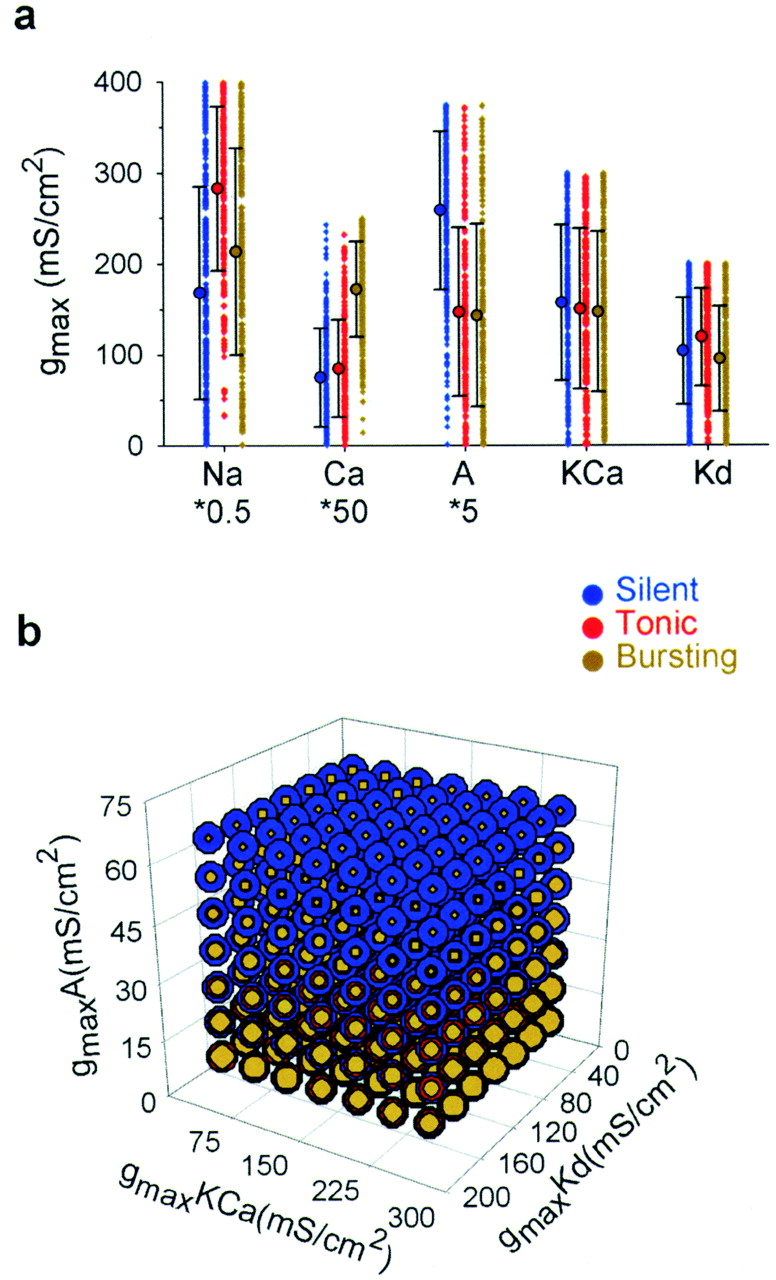
\includegraphics[scale=0.3]{gfx/goldman2001.jpg}
\caption[Dependence of different patterns of activity on ion channel relationships.]{Production of different patterns of activity in the neuron is dependent on the relationship between ion channel maximal conductances. The same maximal conductance density in one ion channel can produce unique patterns of activity dependent on its relationship to other channels. (\textsc{A:}) Different states of activity are observed when ion channel maximal conductances are varied over a wide range. (\textsc{B:}) Different patterns of activity emerge from characteristic sets of K\textsuperscript{+}-type ion channel maximal conductances in a probabilistic manner. The probability of seeing bursting activity, for example, increases as \ac{gA} and \ac{gKd} decrease toward zero\cite{goldman_global_2001}.}
    \label{fig:goldman2005}
\end{figure}

These patterns of correlations in channel expression and conductance density have been proposed reflect the tuning of conductances required to maintain target activity over a long period of time\cite{marder_variability_2006,schulz_variable_2006}.
This may arise during all periods of the life of a neuron, or it may be specific to initial development. In the \ac{STG}, it has been proposed that tuning rules governing development of neurons may result in networks that are highly variable across individuals by the time neural networks are fully developed\cite{marder_development_2005,rehm_spectral_2008,rehm_developmental_2008}.
Furthermore, variability in other systems may induce variability in ion channel expression and current densities -- the variability of transcriptional machinery and regulatory transcriptional sequences can lead to variability in gene transcription, and subsequently ion channel expression\cite{blake_noise_2003,volfson_origins_2006}.
It is currently unknown what biological mechanism, or mechanisms, produce variability across ion channel mRNAs and maximal conductance densities. Though neuroscience has come a long way in understanding how characteristic sets of ion channel mRNAs and maximal conductances can produce similar patterns of activity, we still do not know what drives the existence of these correlations\cite{prinz_similar_2004}.

\subsection{Homeostasis \& Ion Channel Correlations} \label{corr_homeostasis}
The existence of correlations between membrane ion channels may represent a mechanism by which homeostatic regulatory features may enforce and stabilize desired activity in specific neurons\cite{schulz_quantitative_2007}.
Co-regulation of ion channels can theoretically prevent loss of activity while the neuron is being affected by environmental perturbations such as ion channel turnover and activity perturbations\cite{oleary_correlations_2013,maclean_activity-independent_2003,bergquist_hierarchy_2010}.
Characteristic sets of ion channel correlations can consistently produce desired firing rate activity despite high variability in levels of channel conductance densities between individual neurons of the same cell type.
This has been proposed to occur through the enforcement of ion channel ratios, which are correlated to specific activity features. This can simplify homeostatic mechanisms and make the neuron robust to perturbations in any one ion channel\cite{schulz_quantitative_2007,maclean_activity-independent_2005,ball_coregulation_2010,burdakov_physiological_2005}.

Experimental work has shown ion channel correlations to be significantly affected by homeostatic activity\cite{taylor_axonal_2009,tran_ionic_2019,baumgardt_specification_2007,stein_modulation_2009,soofi_co-variation_2012,temporal_neuromodulation_2011}.
For example, MacLean \textit{et al.} showed that modulating \ac{gA} current densities or \ac{gH} current densities alone would change the functional output of the neuron, but that modulating both maintained desired functional output\cite{maclean_activity-independent_2005}.
Along with that, inhibition of \ac{gA} results in compensatory increase in \ac{gKCa} that is dependent on intracellular calcium concentration and calcineurin activity\cite{ransdell_rapid_2012}.
The dependence of this compensatory mechanism on calcium concentration provides evidence that activity-dependent feedback can influence ion channel correlations\cite{turrigiano_activity-dependent_1994,turrigiano_selective_1995}.

Though co-regulation of ion channels provides an avenue by which neurons may maintain desired activity, the mechanism which drives the existence of co-regulation remains a mystery.
Activity-dependent feedback represents but one proposed solution. The mechanism not only influences correlations, but is has been found necessary for the existence of correlated ion channels in the \ac{STG}.
Temporal \textit{et al.} performed experiments decoupling activity, synaptic connectivity, and neuromodulatory states of individual neurons from the \ac{STG}, and found that loss of neuromodulation was not sufficient to result in loss of correlations across channel mRNAs, but loss of activity resulted in loss of all correlations. Thus, it was shown that activity-dependent processes, but not neuromodulatory processes, can dynamically maintain distinct relationships across channel mRNAs in the \ac{STG}\cite{temporal_activity-dependent_2014}.
%TEMPORAL FIGURE
Activity-dependent feedback mechanisms can generate and regulate biophysically realistic dynamics of neurons in the \ac{STG}\cite{oleary_correlations_2013,oleary_cell_2014,liu_model_1998,lemasson_activity-dependent_1993}.
Figure \ref{fig:oleary2013} shows how a model of activity-dependent feedback (described in Section \ref{homeostaticrules}) can produce desired neuronal dynamics by varying channel conductances over time which are dependent on Ca\textsuperscript{2+} dynamics\cite{oleary_correlations_2013}.

\begin{figure}[H]
    \centering
    \includegraphics[width=1.0\linewidth]{gfx/oleary2013.png}
\caption[Model of activity-dependent feedback.]{Development of channel conductances and patterns of activity at different time-points. (\textsc{Left:}) A model of activity-dependent feedback varies channel conductances over time, resulting in desired functional output when channel conductances reach their respective steady-state values. (\textsc{Right:}) Patterns of activity (1-3) correspond to channel conductance values at three points in their evolution over time\cite{oleary_correlations_2013}.}
    \label{fig:oleary2013}
\end{figure}

These mechanisms are able to reliably influence co-regulation of ion channel pairs over different timescales by changing the properties of correlations, including slope, strength, and set-points within the parameter space\cite{stein_modulation_2009,soofi_co-variation_2012,temporal_neuromodulation_2011,tran_ionic_2019}.
%as you can see in this figure... from oleary et al 2013
The key feature of activity-dependent feedback is the dependence of functional output on firing rate activity. To sense changes in firing rate activity, models of activity-dependent feedback must have the capacity to sense these changes.
Calcium dynamics have been proposed as a way neurons can sense changes in activity. Calcium dynamics can indirectly express \ac{Vm} by simulating the interaction between changes in intracellular Ca\textsuperscript{2+} concentration and changes in \ac{Vm}.

Modern models of homeostasis typically use calcium dynamics as a sensor by which neurons can regulate activity\cite{turrigiano_activity-dependent_1994,turrigiano_selective_1995,oleary_correlations_2013,liu_model_1998}.
Changes in intracellular Ca\textsuperscript{2+} concentration can be averaged over different timescales in order to target different aspects of firing rate activity\cite{liu_model_1998}. In doing so, neurons can assure that functional output is properly maintained.
Liu \textit{et al.} described how different patterns of activity can have average Ca\textsuperscript{2+} concentration levels that may be difficult to differentiate between.

\begin{figure}[H]
    \centering
    \includegraphics[scale=0.7]{gfx/liu1998}
    \caption[Activity pattern differentiation in a single Ca\textsuperscript{2+} sensor setup.]{Three different patterns of activity have effectively equal average Ca\textsuperscript{2+}. (\textsc{A:}) \ac{Vm} of a neuron firing tonically. (\textsc{B:}) \ac{Vm} of a neuron firing with bursting behavior. (\textsc{C:}) \ac{Vm} of a neuron firing with a different bursting behavior. (\textsc{All, Right:}) Instantaneous Ca\textsuperscript{2+} concentration and respective time-averaged values\cite{liu_model_1998}.}
    \label{fig:liu1998}
\end{figure}

Figure \ref{fig:liu1998} shows that the Ca\textsuperscript{2+} average levels averaged over a single timescale across a tonic firing pattern and two separate bursting patterns are effectively equal. This shows that neurons which use a single Ca\textsuperscript{2+} sensor averaged over one unique timescale can, in theory and in some cases, not differentiate between different patterns of activity.
In contrast, Figure \ref{fig:liu1998_2} describes the use of three separate Ca\textsuperscript{2+} sensors which can distinguish between different activity patterns by averaging intracellular Ca\textsuperscript{2+} concentration over three distinct timescales.
The use of three sensors is not arbitrary in this case, but targets three key features of the neuron's electrophysiology. The fast Ca\textsuperscript{2+} sensor is able to detect tonic firing patterns, the slow Ca\textsuperscript{2+} sensor is able to detect bursting behavior, and the DC Ca\textsuperscript{2+} sensor can detect slow-wave activity.

\begin{figure}[H]
    \centering
    \includegraphics[scale=0.5]{gfx/liu1998_2.png}
    \caption[Activity pattern differentiation in a multiple Ca\textsuperscript{2+} sensor setup]{Three different Ca\textsuperscript{2+} sensors can differentiate between different patterns of activity. Rows \textsc{A-C} are the same activity patterns found in Figure \ref{fig:liu1998}. Second column shows Ca\textsuperscript{2+} current. Last three columns show transient and average values for three different Ca\textsuperscript{2+} sensors: Fast, Slow, and DC\cite{liu_model_1998}.}
    \label{fig:liu1998_2}
\end{figure}

Despite this, models of activity-dependent feedback have been produced which can differentiate between different patterns of activity, and reliably produce target behavior from initial conditions which produce quiescent behavior\cite{oleary_correlations_2013,oleary_cell_2014}. O'Leary \textit{et al.} has proposed a model which relies on a single Ca\textsuperscript{2+} sensor. At each discrete time-step, the difference, or "error," between the average Ca\textsuperscript{2+} concentration and the target Ca\textsuperscript{2+} concentration is computed, and integrated with past computations of error\cite{oleary_cell_2014}. This is then fed into two differential equations, one of which represents the synthesis of correlated ion channel mRNAs, and the other represents translation of ion channel proteins from the current channel mRNA concentration. This model scales the average Ca\textsuperscript{2+} concentration at the level of mRNA transcription, rather than at the level of the Ca\textsuperscript{2+} sensor. Ratios between ion channel maximal conductances can then specify correlations between conductances, and in turn specify the pattern of activity of the neuron. This model is shown to be a perfect candidate for exploring the effect of variability in other properties of the neuron on the variability of ion channel mRNA concentrations and maximal conductance densities.

Despite these significant achievements in producing biophysically realistic models of neuronal dynamics and homeostatic activity, ion channel correlations have nonetheless proven a significant challenge to models of neurons with homeostatic regulation. Sets of correlations are dissimilar across cell types and highly variable within cell types, making generalizability a challenge. Without an understanding of the functional mechanism driving their existence, or the biological mechanisms underlying activity-dependent feedback, creating biophysically realistic models is even more difficult\cite{schulz_quantitative_2007}.
The experimentally-derived correlations between ion channels have, as of now, not been successfully reproduced in models of homeostatic regulation\cite{schulz_variable_2006,schulz_quantitative_2007,oleary_correlations_2013,oleary_cell_2014,liu_model_1998}.
The model by O'Leary \textit{et al.} described above is capable of producing linear pairwise correlations between ion channel maximal conductances, but has not been able thus far to produce the non-binary patterns of correlations seen in Figure \ref{fig:santinschulz2019}\cite{oleary_cell_2014}.

In this thesis, variability in properties of model neurons including initial channel maximal conductances and mRNA levels, \acf{gleak}, \acf{taum}, \acf{taug}, and \acf{Ca_target} will be varied independently and systematically examined. The purpose in doing this is to understand the influence of intrinsic neural parameters and parameters of homeostatic regulation on emergence of ion channel correlations and the possible ways neurons can manifest ion channel correlations which are as diverse and robust as is seen in experimental observations.\cite{schulz_variable_2006,schulz_quantitative_2007}.


\cleardoublepage
\ctparttext{You can put some informational part preamble text here.
Illo principalmente su nos. Non message \emph{occidental} angloromanic
da. Debitas effortio simplificate sia se, auxiliar summarios da que,
se avantiate publicationes via. Pan in terra summarios, capital
interlingua se que. Al via multo esser specimen, campo responder que
da. Le usate medical addresses pro, europa origine sanctificate nos se.}
\part{The Showcase}\label{pt:showcase}
%************************************************
\chapter{Methods}\label{ch:methods}
%************************************************

This thesis relies on a previously described model of a neuron. It is a single-compartment, conductance-based neuron which is based on the Hogkin-Huxley formalism\cite{hodgkin_components_1952,hodgkin_measurement_1952,hodgkin_quantitative_1952}. Previous work has utilized this model neuron as a backbone for exploration of homeostatic compensatory mechanisms\cite{oleary_correlations_2013,oleary_cell_2014,liu_model_1998}.
This model represents the neuron as a circuit\cite{hodgkin_quantitative_1952}. Figure \ref{fig:hhcircuit} details the circuit diagram of the neuron as a representation of the cell membrane acting as a capacitor with various ion channels as resistors. The membrane takes in current from the outside, which can be described in more detail as the neuron's neuromodulatory environment.

\begin{figure}[h]
    \centering
    \includegraphics[angle=0.75,width=\linewidth]{gfx/hodgkinhuxleycircuit.png}
    \caption[Circuit diagram representing membrane of a neuron.]{Circuit diagram representing the membrane of a neuron. \ac{Cm} represents the total capacitance of the neuron. Resistors represent \(1/\acs{gNaV}\), \(1/\acs{gK}\), and \(1/\ac{gleak}\)\cite{hodgkin_quantitative_1952}.}
    \label{fig:hhcircuit}
\end{figure}

The model neuron has eight transmembrane currents and associated conductances: \acf{INaV}, \acf{IA}, \acf{IH}, \acf{IKCa}, \acf{IKd}, \acf{ICaS}, \acf{ICaT}, and \acf{Ileak}.
The associated maximal conductances of the first seven transmembrane currents are regulated by the integral control scheme mentioned in Section \ref{homeostaticrules}. \ac{gleak} is not regulated in this model.

\section{Neurodynamics} \label{neurodynamics}

Neurons are considered to consist of a single compartment, acting as a capacitor, with various ionic currents acting as resistors in parallel, and a specific surface area (in units $mm^2$).
The compartment has a \acf{Vm}, which evolves according to the equation:

\begin{equation} \label{eq:voltage}
C_m \frac{\mathrm{d}V_m}{\mathrm{d}t} = \sum_{i} I_i
\end{equation}

where $\acs{Cm}$ is the specific capacitance of the membrane and $I_i$ is each ionic current in the neuron\cite{gorur-shandilya_xolotl_2018}. Current is given by the equation

\begin{equation} \label{eq: current}
    I_i = g_i(V)(V - E_i)
\end{equation}

where $g_i(V)$ is instantaneous conductance and $E_i$ is the reversal potential (Nernst potential) for each ion channel\cite{gorur-shandilya_xolotl_2018}. Reversal potentials for each ion channel, excluding Ca\textsuperscript{2+}-dependent channels, are considered constant and are described in Section \ref{modelparameters}. This simplification is justified by the law of large numbers -- intracellular and extracellular ion concentration are saturated, resulting in effectively constant flux of ions in and out of the cell\cite{liu_model_1998}. Instantaneous conductance $g_i(V)$ is defined by the equation:

\begin{equation} \label{eq: conductance}
    g_i(V) = \bar{g_i} m_i^{p_i} h_i^{q_i}
\end{equation}

where

\begin{tabular}{ll}
    $\bar{g_i}$     & maximal conductance for each ion channel \\
    $m$             & activation gating variable \\
    $h$             & inactivation gating variable \\
    $p, q$          & integers \\
\end{tabular}

The integers $p$ and $q$ are bound by an interval $[0,1]$\cite{gorur-shandilya_xolotl_2018}. The activation and inactivation variables are themselves defined by an ordinary differential equation which depends on \ac{Vm}, and is specific to each conductance. The general form is:

\begin{align}
    \tau_m \frac{\mathrm{d}m}{\mathrm{d}t} = m_\infty - m \\
    \tau_h \frac{\mathrm{d}h}{\mathrm{d}t} = h_\infty - h
\end{align}

where $\tau_m$ and $\tau_h$ are time constants and $m_\infty$ and $h_\infty$ are steady-state values of the activation and inactivation variables\cite{prinz_alternative_2003}. Each conductance has a characteristic steady-state density and time constant which represent its function in the overall neurodynamics of the neuron.

\section{Homeostatic Rules}\label{homeostaticrules}

Regulation of firing rate activity in this thesis will rely on an activity-dependent feedback mechanism for regulating ion channel maximal conductances\cite{oleary_correlations_2013,oleary_cell_2014,liu_model_1998,prinz_alternative_2003}.
This mechanism relies on calcium as a sensor, by which neurons may regulate their activity. Section \ref{corr_homeostasis} provides an explanation of the use of calcium ions as an indirect representation of \ac{Vm} activity.
Calcium dynamics in this model evolve according to the equation:

\begin{equation} \label{eq:calcium}
    \tau_{Ca} \frac{\mathrm{d}[Ca^{2+}]}{\mathrm{d}t} = -f(I_{CaT} + I_{CaS}) - [Ca^{2+}] + [Ca^{2+}]_0
\end{equation}

where $\tau_{Ca}$ is the time constant, $f$ translates $Ca^{2+}$ current into an intracellular concentration change, and $[Ca^{2+}]_0$ is the steady state intracellular $Ca^{2+}$ concentration if there is no flux of calcium ions across the membrane\cite{prinz_alternative_2003,liu_model_1998}.

The activity-dependent feedback mechanism is based on regulation by a calcium-dependent homeostatic rule, first implemented by O'Leary \textit{et al.}\cite{oleary_cell_2014}.
Regulation of maximal conductances is simulated by two integral control equations:

\begin{align} \label{eq:integralregulation}
    \tau_i \dot{m_i} &= [Ca^{2+}] - Ca_{tgt} \\
    \label{eq:integralregulation2}
    \tau_g \dot{g_i} &= m_i - g_i
\end{align}

where $\tau_i$ represents the transcription timescale for each ion channel, $\tau_g$ represents global transcription timescale, $m_i$ represents mRNA levels for each ion channel, and $Ca_{tgt}$ represents global Ca\textsuperscript{2+} target concentration. Variables are bounded at 0 to ensure that conductances do not become negative.

In this model, $Ca^{2+}$ acts as a feedback control signal. It is purposefully simple, focusing on the essential biological principles underlying formation and degradation of ion channel proteins. Obviously, neurons possess a significant number of other mechanisms of regulation, such as co-trafficking of ion channels, cotranslational interaction, RNA interference, and the use of promoters\cite{oleary_cell_2014,shi_subunits_1996,vanoye_kcnq1/kcne1_2010,arcangeli_ion_2011,frank_endogenous_2011,zhang_recovery_2011}. Occam's razor dictates that "the simplest solution is most likely the right one," and we will use this as a guideline moving forward.

Steady-state values of $m_i$ are found to be dependent on the time integral of average $[Ca^{2+}]$ and scaled by the inverse of the time constant for the channel $\tau_i$. We can then estimate steady state $g_i$ for very small initial conductance values and positive time constants. We can see this by taking the integral of Equation \ref{eq:integralregulation}:

\begin{equation} \label{eq:steadystateg}
    g_i \approx m_i = \frac{1}{\tau_i} \int_{0}^{t_{ss}} ([Ca^{2+}] - Ca_tgt)dt
\end{equation}

Figure \ref{eq:steadystateg} also shows how correlations between ion channels emerge when $m_i$ converges to the value dependent on the time integral of average $[Ca^{2+}]$. When one takes ratios between channels, the integrals cancel out, so that:

\begin{equation}
    \frac{g_i}{g_j} \approx \frac{\tau_j}{\tau_i}
\end{equation}

It can be seen here that different ratios of the time constants determine the correlations between ion channel conductances. These ratios can determine the electrophysiological character of the neuron, as is further discussed in Section \ref{corr_homeostasis}.

\section{Model Parameters} \label{modelparameters}

Model parameters are adapted from previous work, and are used as the basis for variation in each experiment presented in this thesis\cite{prinz_alternative_2003,oleary_cell_2014,liu_model_1998}.

Each ionic current has its own reversal potential. These values dictate the membrane potential at which ions begin to move in the opposite direction.

\begin{table}[h]
    \centering
    \begin{tabular}{ccccccccc}
         \textsc{Current} & \ac{INaV} & \ac{IA} & \ac{IH} & \ac{IKd} & \ac{IKCa} & \ac{Ileak} \\
         \hline
         $E \mathrm{(mV)}$ & +50 & -80 & -20 & -80 & -80 & -50
    \end{tabular}
    \caption[Reversal potentials for each ion channel.]{Reversal potential for each ionic current. Reversal potential of \ac{ICaT} and \ac{ICaS} are not constant and derived from the Nernst potential.\cite{prinz_alternative_2003}}
    \label{tab:revpotential}
\end{table}

\ac{Vm} evolves with time according to Equation \ref{eq:voltage} where specific membrane capacitance $C_m = 0.628nF$\cite{hodgkin_quantitative_1952}.

Ca\textsuperscript{2+} concentration is dynamic, evolving according to Equation \ref{eq:calcium}, where

   \begin{tabular}{l}
     $\tau_{Ca} = 200ms$ \\
     $f = 14.96 \mu M/nA$
    \end{tabular}
    
$\tau_{Ca}$ is the calcium buffering time constant, and $f$ is the factor which converts calcium current into intracellular calcium concentration change. This factor depends on the ratio of the surface area of the cell to the volume wherein Ca\textsuperscript{2+} concentration is measured\cite{liu_model_1998}. In this case, volume is considered to be a narrow shell inside the membrane and approximates the neuron by a cylinder $50 \mu m$ in diameter and $400 \mu m$ long. Surface area of the cell is 0.0628 mm\textsuperscript{2}\cite{liu_model_1998}.

Reversal potentials of Ca\textsuperscript{2+} current types are dependent on voltage and calcium, and are dynamically updated by the Nernst equation\cite{liu_model_1998}:

\begin{equation}
    E_{Ca} = \frac{RT}{zF} ln(\frac{[Ca^{2+}]_{ext}}{[Ca^{2+}]_{in}}
\end{equation}

where $E_{Ca}$ refers to reversal potentials for \ac{ICaS} and \ac{ICaT}, gas constant $R = 8.314 J*mol/K$, temperature $T = 284.15 K$, ion charge $z = 2$ for calcium ions, Faraday constant $F = 96485 C/mol$, $[Ca^{2+}]_{in}$ is the current intracellular calcium concentration, and the extracellular calcium concentration $[Ca^{2+}]_{ext} = 0.05 \mu M$\cite{prinz_alternative_2003}.

Voltage-dependent equations for the model parameters for each current were adapted from \cite{prinz_alternative_2003}. Each ionic current has its own specific $p$, steady-state activation variable $m_\infty$, steady-state inactivation variable $h_\infty$, and time constants $\tau_m$ and $\tau_h$, respectively. Ionic currents which are not inactivating do not have values for $h_\infty$ or $\tau_h$.

Maximal conductances are dependent on Ca\textsuperscript{2+} concentration and are regulated by Equations \ref{eq:integralregulation} and \ref{eq:integralregulation2}. The time constant for transcriptional rate $\tau_{m_i}$ is unique for each maximal conductance and defined by:

\begin{equation}
    \tau_{m_i} = \frac{5e6}{g_{\infty_i}}
\end{equation}

where $tau_m$ is in milliseconds and $g_{i\infty}$ represents the steady-state maximal conductance for each ionic channel. Steady-state maximal conductances were originally adapted from Prinz \textit{et al.}\cite{prinz_alternative_2003}.

\begin{table}[H]
    \centering
    \begin{tabular}{ccccccccc}
        \textsc{Ion channel} & NaV & CaT & CaS & A & H & KCa & Kd & Leak \\
        \hline
    $g_\infty$ $(\mu S/mm^2)$ & $1e3$ & $25$ & $60$ & $5e2$ & $0.1$ & $50$ & $1e3$ & $*$ \\
        \hline
        $\tau_m$ $(ms)$ & $5e3$ & $2e5$ & $\approx 8.33e4$ & $1e4$ & $5e7$ & $1e5$ & $5e3$ & $*$ \\
        \hline
        $\tau_g$ $(ms)$ & $5e3$ & $5e3$ & $5e3$ & $5e3$ & $5e3$ & $5e3$ & $5e3$ & $*$
    \end{tabular}
    \caption[Integral control model parameters]{Default integral control model parameters. $g_\infty$ adapted from Prinz \textit{et al.} to determine transcriptional rate time constants $\tau_m$ for each ionic current\cite{prinz_alternative_2003}. Translation rate time constant $\tau_g$ is equal across all ionic currents. *Leak is unregulated in this model and thus does not have $\tau_m$ or $\tau_g$ time constants.}
    \label{tab:integralparameters}
\end{table}

Table \ref{tab:integralparameters} describes the regulation time constants used in both Equations \ref{eq:integralregulation} and \ref{eq:integralregulation2}. Steady state maximal conductances ($g_\infty$) were computed by simulating a known working set of eight channel maximal conductances adapted from Prinz. \textit{et al.} for $t = 400s$ with a time-step of $dt = 0.1ms$ to ensure all maximal conductances converged at their respective steady state densities\cite{prinz_alternative_2003}. These values are only used to compute the transcription and translation rate time constants, and are not used at any point after these values are calculated. It should be of note that these time constants are the default for all experiments, except in cases where the time constants are being varied themselves. In that case, these default values are used as a median point upon which to build a distribution. Target Ca\textsuperscript{2+} concentration was established for a bursting neuron through this same method. Average Ca\textsuperscript{2+} concentration, averaged over 200ms, was obtained from the model after simulation. Initialization of Ca\textsuperscript{2+} target concentration and regulation time constants was repeated at the beginning of each experiment. 

\section{Simulating Neurons}

Model neurons are simulated according to the exponential Euler method,\cite{gorur-shandilya_xolotl_2018,dayan2001theoretical} which approximates \ac{Vm} at each discrete time step by the equation:

\begin{equation} \label{eq:expeuler}
V(t + \mathrm{d}t) = V_\infty + (V(t) - V_\infty)exp(-\frac{\mathrm{d}t}{\tau_V})
\end{equation}

Neurons are simulated for $t = 200s$ with a timestep of $dt = 0.1ms$. Voltage traces used for figures and metrics are computed by simulating model neurons for $t = 6s$ with a timestep of $dt = 0.1ms$.

The homeostatic mechanism is simulated by the Euler method\cite{gorur-shandilya_xolotl_2018}:

\begin{align} \label{eq:integraleuler}
    Ca_{err} &= Ca_{tgt} - Ca_{prev} \\
    m_i(t+\mathrm{d}t) &= m_i + \frac{\mathrm{d}t}{\tau_{m_i}}Ca_{err} \\
    \bar{g}_i(t+\mathrm{d}t) &= \bar{g}_i + \frac{\mathrm{d}t}{\tau_{g_i}}(m_i - \bar{g}A)
\end{align}

where $m_i$ represents ion channel mRNA concentration for each current, $\bar{g}_i$ represents maximal conductance density for each current, $Ca_{tgt}$ represents target average Ca\textsuperscript{2+} concentration, $Ca_{prev}$ represents Ca\textsuperscript{2+} concentration at the previous time-step, and $A$ represents the surface area of the model neuron.

\section{Initial Conditions} \label{initialconditions}

Model compartments are initialized with parameters $\ac{Vm} = -60 mV$ and $[Ca^{2+}_{in}] = 0.05 \mu M$.
Initial maximal conductances ($\mu S/mm^2$) for each channel (excluding \ac{gleak}) and compartment mRNA concentration ($\mu M$) are varied across all experiments. \ac{gleak} is held fixed at $\bar{g}_{leak} = 0.05$, except in Figure \ref{fig:integralvariation_Leak}.
Values are generated for all simulations at the beginning of each experiment by the use of a random number generator scaled by a noise factor.
For the first experiment, where initial conditions are varied alone, the noise factor is $20$ for channel maximal conductances and $0.004$ for compartment mRNA concentration. For all other experiments, the noise factor is $5$ for channel maximal conductances and $0.001$ for mRNA levels.

\section{Activity Metrics} \label{electrophys}

For each simulation, metrics were computed on model parameters to determine if models were working or not. Models were considered to have converged if

\begin{equation}
    \mid \frac{([Ca_{tgt}] - [Ca_{avg}])}{[Ca_{tgt}]} \mid > 0.1
\end{equation}

where $Ca_{tgt}$ is the target Ca\textsuperscript{2+} concentration and $Ca_{avg}$ is the average Ca\textsuperscript{2+} concentration after homeostatic regulation.

Models were then checked against reference model with parameters described in Table \ref{tab:integralparameters}. Burst periods and duty cycle were checked against reference model. If the burst period of the tested model deviated from reference by more than 20\% or the duty cycle deviated from reference more than 10\%, the model was considered nonfunctional.

\section{Model Implementation} \label{implementation}

Model neurons were implemented using \texttt{xolotl} v.20.4.22 and v.20.2.26, an open-source neuron simulator written in C++ for MATLAB\cite{gorur-shandilya_xolotl_2018}. Credit to Srinivas Gorur-Shandilya for development and implementation of the modeling platform. Simulation data was retrieved through the use of MATLAB ver. R2020a.





%\addtocontents{toc}{\protect\clearpage} % <--- just debug stuff, ignore
%************************************************
\chapter{Results}\label{ch:results}
%************************************************

How do homeostatic tuning rules produce variability and correlations between ion channel conductances and mRNA levels in neurons? To answer this question, we will vary intrinsic properties of a model neuron and properties of a homeostatic tuning rule to ascertain the influence of these parameters on the emergence of correlations between ion channels in neurons.
We began with a conductance-based model neuron based on the Hogkin-Huxley formalism that was modified to take advantage of a homeostatic compensatory mechanism. Model neurons utilize intracellular Ca\textsuperscript{2+} concentration as a sensor to regulate conductance values of individual ion channels. These neurons are thus indirectly dependent on \ac{Vm} via the dependence of Ca\textsuperscript{2+} dynamics on \ac{Vm}\cite{oleary_correlations_2013,liu_model_1998}.
This model produces and maintains complex activity patterns, such as tonic firing and bursting behavior, through the interplay between target Ca\textsuperscript{2+} concentration, Ca\textsuperscript{2+} dynamics, and voltage-dependent ion channels.

We will utilize an integral control model, based off of the mechanism proposed by O'Leary \textit{et al.} which utilizes a single Ca\textsuperscript{2+} sensor to regulate channel mRNA levels and maximal conductances based on firing rate activity.\cite{oleary_correlations_2013}.
Rate of regulation of maximal conductance values by the homeostatic rule is based on experimental work suggesting that regulatory dynamics occur over hours or even days\cite{desai_homeostatic_2003,davis_homeostatic_2006,turrigiano_homeostatic_1999}.
Of course, simulating the evolution of neurodynamics over a period of hours or even days is computationally inefficient, so both the time of integration and regulatory timescales have been scaled down to a more appropriate 200 seconds for each simulation.

\begin{figure}[h]
    \centering
    \includegraphics[width=1.0\linewidth]{gfx/development.png}
\caption[Development of an integral control model.]{An integral control scheme with one Ca\textsuperscript{2+} sensor can produce bursting behavior after homeostatic regulation. \textsc{(Top:)} Development of maximal conductances from initial conditions. \ac{gleak} is excluded as it is not regulated. (\textsc{Bottom, left:}) Quiescent behavior in model neuron prior to homeostatic regulation. (\textsc{Bottom, right:}) Bursting behavior of model neuron after t = 200 seconds. Integral control scheme adapted from \cite{oleary_correlations_2013}.}
    \label{fig:integraldevelopment}
\end{figure}

Figure \ref{fig:integraldevelopment} shows the development of maximal conductances over time. Each individual line in the top section of the figure corresponds to the development of each ion channel maximal conductance. The bottom section shows the functional output of the model before and after homeostatic regulation. Quasi-random initial conditions were generated for initial maximal conductances and ion channel mRNA levels. The model was then allowed to develop in an unconstrained manner for a set period of time ($t = 200 s$).

%% EXPAND THE FIGURE TO USE TONIC SPIKING TOO!!!
We wanted to understand not only how neurons are capable of producing correlations between ion channels, but how variability in the scale and connection strengths of correlations was produced by homeostatic regulation.
We assumed that variability in scale and connection strengths of ion channel correlations is not dependent on the intrinsic parameters of the neuron, but rather the parameters of the homeostatic tuning rule.
To answers these questions, we will start by varying initial conditions (channel maximal conductances and mRNA levels) of the model neuron. Then, we will vary \acf{gleak}, as it is not regulated by the homeostatic tuning rule.
Then, we will vary parameters in the homeostatic tuning rule, including Ca\textsuperscript{2+} target concentration, \acf{taug}, and \acf{taum}.
Taking into account how variation in intrinsic model neuron parameters affects patterns of correlation, we will systematically examine how variation in these parameters changes the patterns of correlations between steady state channel maximal conductances to ascertain the influence of each parameter on the emergence of ion channel correlations in neurons.

Before modulating the individual parameters of the model, we wanted to recapitulate that the model was capable of producing similar patterns of activity from significantly different sets of initial channel maximal conductances\cite{oleary_cell_2014}. We initialized two sets of 1000 model neurons each with initial maximal conductance values that differed by 100-fold between distributions. We set target Ca\textsuperscript{2+} concentration to be the reference value for a bursting neuron obtained from the database produced by Prinz \textit{et al.} and described in Section \ref{initialconditions}\cite{prinz_alternative_2003}. We then simulated unconstrained homeostatic regulation for each model neuron for $t = 200s$. We filtered out models where maximal conductances had not converged to steady state, or had bursting periods and duty cycles that differed significantly from the reference model, as further described in Section \ref{electrophys}. Figure \ref{fig:var_integral} shows the mean values of each ion channel maximal conductance before and after homeostatic regulation for both sets of model neurons. It is shown that despite a 100-fold difference in initial ion channel maximal conductances between sets, the same pattern of steady state maximal conductances emerges after homeostatic regulation in each set of model neurons.

\begin{figure}[H]
    \centering
    \includegraphics[scale=0.2]{gfx/varboth.png}
\caption[Mean ion channel conductances of \ac{g0} and steady-state maximal conductance values in an integral control model.]{A characteristic set of mean steady state maximal conductances (orange) emerges from two significantly different sets of initial mean maximal conductances (blue).  Despite a 100-fold difference between the two distributions of initial maximal conductances, a strikingly similar set of steady-state maximal conductances is produced in both cases. Initial conditions were generated by a random number generator scaled by a factor of (\textsc{A:}) 1000 and (\textsc{B:}) 100. Note that \ac{gH} is present, but of significantly lower value than other maximal conductances.}\label{fig:var_integral}
\end{figure}

\section{Variability in Initial Conditions of Model Neurons}

After establishing that the model could reproduce characteristic sets of channel maximal conductances for a target behavior, we wanted to explore the correlations between ion channels after homeostatic regulation. Figure \ref{fig:integralcorrelations} shows how pairwise correlations between ion channels emerge from homeostatic regulation utilizing the same integral control scheme described above. 1000 model neurons were initialized with quasi-random initial ion channel maximal conductances varying between [0,5]. After homeostatic regulation, all steady state maximal conductances converge to a single common plane, indicating that the solution set of all channel maximal conductances that produce target activity can be derived from further analysis of this plane.
Furthermore, ion channel maximal conductances in this model are perfectly correlated when initial channel maximal conductances and channel mRNA concentrations are varied by a small degree. It was seen that despite maximal conductances between ion channels existing at different scales, regulated by their individual regulation time constants, an increase in one ion channel maximal conductance is matched by all others at an equal rate.

\begin{figure}[H]
    \centering
    %\begin{addmargin}[-2.5cm]{-3cm}
    \begin{minipage}{\textwidth}
    \centering
    \includegraphics[scale=0.5]{gfx/olearycorrg0.png}
    \end{minipage}
%\end{addmargin}
    %\begin{addmargin}[-2.5cm]{-3cm}
    \begin{minipage}{\textwidth}
    \centering
    \includegraphics[scale=0.5]{gfx/olearycorrmax.png}
    \end{minipage}
    %\end{addmargin}
    
\caption[Correlations between ion channels after homeostatic regulation.]{Pairwise correlations between ion channel maximal conductances ($\mu S/mm^2$) emerge from a homeostatic regulatory mechanism with one Ca\textsuperscript{2+} sensor. Range of variation for each maximal conductance is less than what has been established in experimental observations\cite{golowasch_activity-dependent_1999}. Sets of initial maximal conductances between [0,5] and compartment mRNA concentration between [0,0.001] are not sufficient to reproduce experimentally observed variation in maximal conductances. This small variation in initial conditions reproduces the linear pairwise correlations between steady state maximal conductances seen in \cite{oleary_cell_2014}. Each data point represents ion channel maximal conductances from one simulation. (\textsc{A:}) Pairwise correlations in initial maximal conductances between ion channels. (\textsc{B:}) Pairwise correlations in steady-state maximal conductances between ion channels.}
    \label{fig:integralcorrelations}
\end{figure}
 
This result was expected. However, in experimental observations of correlations between channel mRNA concentrations, pairwise correlations between mRNA levels vary several-fold, and have diverse connection strengths which do not result in perfectly correlated steady state maximal conductances. Pairwise correlations between channel mRNAs do not, in all cases, vary at the same rate as each other, and some channels are not correlated at all\cite{santin_membrane_2019}.


\begin{figure}[H]
	\centering
	\begin{addmargin}[-2cm]{-3cm}
	\includegraphics[scale=0.4]{gfx/fullfigmRNA.png}
	\end{addmargin}
\caption[Variability in initial maximal conductances and mRNA levels under integral control.]{Variability in initial maximal conductances and channel mRNA concentration is not sufficient to reproduce experimentally observed variation in maximal conductances. Coefficient of variation (CV) for initial \ac{gA} is $0.58$, and for steady state \ac{gA} is $0.0030$. The homeostatic rule is shown here to compress variability in maximal conductances by a factor of 190 when initial maximal conductances and compartment mRNA levels are varied by a factor of 20 and 0.004, respectively. (\textsc{A:}) Voltage trace of model neuron prior to integration shows quiescent behavior. (\textsc{B:}) Voltage trace of model after integration shows bursting behavior. (\textsc{C:}) Pairwise correlations between \ac{gA} and \ac{gCaS} prior to integration. (\textsc{D:}) Pairwise correlations between \ac{gA} and \ac{gCaS} after integration. Linear fitting revealed \(R\textsuperscript{2} = 0.991\), indicating \ac{gA} and \ac{gCaS} are highly correlated. Histograms in both pairwise correlation plots show the distribution of maximal conductances for both \ac{gA} and \ac{gCaS}. (\textsc{E:}) Variability in initial compartment mRNA level concentration of \ac{gA} vs. variability in \ac{gA}. Variability in \ac{gA} increases with variability in \ac{gA} channel mRNA concentration at a rate significantly lower than \ac{gA} channel mRNA concentration  alone. (\textsc{F:}) Number of functional models vs. variability in \ac{gA} channel mRNA concentration.}
\label{fig:integralvariation_g0}
\end{figure}

It was then hypothesized that the scale of variability in initial maximal conductances and mRNA levels could contribute to patterns of ion channel correlations. We increased the variability in initial maximal conductances by a factor of 100, and in mRNA levels by a factor of 50. 1000 model neurons were initialized to quasi-random initial maximal conductances ranging between [0,500] and initial channel mRNA concentrations ranging between [0,0.05].
Figure \ref{fig:integralvariation_g0} shows the results of this experiment. It was found that a larger variation in initial conditions was not sufficient to reproduce the linear pairwise correlations between steady state channel maximal conductances, nor the variability in connection strengths observed experimentally. This indicated that initial conditions of the model neuron were not a significant influence on the emergence of ion channel correlations. Each model neuron underwent homeostatic regulation for $t = 200s$. As performed before, each model neuron was checked to ensure that the model converged to steady state maximal conductances, and had behavioral features which did not significantly differ from the reference bursting model neuron. The majority of model neurons produced target bursting behavior, showing that the integral control scheme is highly resistant to variation in these parameters. We can see that variability in maximal channel conductances increases with variability in channel mRNA concentration at a rate far lower than mRNA concentration alone. Most importantly, it was found that variability in these parameters resulted in compression of pairwise correlations between steady state maximal conductances from initial maximal conductances by a factor of 190, and that all versions of the model lie on a single point of the plane.
%with a success rate of \textbf{\textbf{\textbf{\textbf{insert}}}}

\section{Variability in Passive Ion Leak Conductance}

We then moved on \acf{gleak}, which is unregulated in this model. It was hypothesized that though variability in regulated model parameters was insufficient to reproduce experimentally observed correlations, \ac{gleak} may have a significant influence because it is not regulated by the homeostatic rule.

Given that initial maximal conductances and channel mRNA concentrations were insufficient to reproduce experimentally observed variability in steady state channel maximal conductances, these parameters were allowed to vary between [0,5] and [0,0.001], respectively. \ac{gleak} was varied between [0,0.2] across all model neurons. \ac{gleak} was bound at 0.2 as the number of functional models after homeostatic regulation decreased significantly past this point.

\begin{figure}[H]
    \centering
    \begin{addmargin}[-2cm]{-3cm}
    \includegraphics[scale=0.4]{gfx/fullfigLeak.png}
    \end{addmargin}
\caption[Variability in \ac{gleak} under integral control.]{Variability in \ac{gleak} reproduces linear pairwise correlation between \ac{gA} and \ac{gCaS}. However, variation in maximal conductances is less than two-fold. CV for initial \ac{gA} is $0.583$ and for steady state \ac{gA} is $0.00301$, resulting in a compression factor of 120 when varying \ac{gleak} between [0,0.2]. (\textsc{A-D:}) Same as Figure \ref{fig:integralvariation_g0}. Linear fitting revealed \(R\textsuperscript{2} = 1\), indicating \ac{gA} and \ac{gCaS} are perfectly correlated. (\textsc{E:}) Variability in \ac{gleak} vs. variability in \ac{gA}. Variability in \ac{gA} increases with variability in \ac{gleak} at a rate significantly lower than \ac{gleak} alone. (\textsc{F:}) Number of functional models vs. variability in \ac{gleak}.}
    \label{fig:integralvariation_Leak}
\end{figure}

Figure \ref{fig:integralvariation_Leak} shows the results of the experiment. In stark contrast to a comparatively large variation in initial maximal conductances and channel mRNA levels, variation in \ac{gleak} was able to reproduce linear pairwise correlations between \ac{gA} and \ac{gCaS}. All solution sets of steady states maximal conductances in this experimental paradigm lie on a single plane taking the form of a line. However, despite greater than two-fold variability in \ac{gleak}, variation in steady state channel maximal conductances was less than two-fold, and was significantly compressed by the homeostatic rule with a compression factor of 120 between initial \ac{gA} and \ac{gA} after homeostatic regulation. Furthermore, variation in \ac{gA} increased at a rate significantly lower than \ac{gleak}, further cementing the compression in variability the homeostatic rule produced. It was determined that \ac{gleak} has a minor influence on the patterns of ion channel correlations that emerge from homeostatic regulation, but that variability in \ac{gleak} alone is not sufficient to reproduce the scale of variability in experimentally observed correlations, nor the variability in connection strengths between maximal conductances.

\section{Variability in Target Ca\textsuperscript{2+} Concentration}

We then examined the features of the homeostatic tuning rule itself. We started off by varying \ac{Ca_target}, positing that individual neurons may possess unique variability in target calcium concentration that can result in experimentally observed patterns of correlations while still producing target behavior. The experiment was set up in the same way as the previous experiment, with the same variation allowed in initial channel maximal conductances and mRNA concentrations. The distribution of \ac{Ca_target} values was produced by scaling the reference value obtained from the Prinz \textit{et al.} database described previously, and scaling it by a factor of 30. This scaling factor was produced by fine-tuning variation to ensure that a significant number of model neurons converged to bursting behavior after homeostatic regulation, but made sure that not all models converged so as to see the extreme ends of variation in this target.

%CV LEFT = 0.56 CV RIGHT = 0.0464
\begin{figure}[H]
    \centering
    \begin{addmargin}[-2cm]{-3cm}
    \includegraphics[scale=0.4]{gfx/fullfigCa.png}
    \end{addmargin}
\caption[Variability in \acs{Ca_target} under integral control.]{Variability in \ac{Ca_target} reproduces linear pairwise correlation between \ac{gA} and \ac{gCaS}. Both \ac{gA} and \ac{gCaS} are shown to vary approximately two-fold, which is consistent with experimental evidence.\cite{golowasch_activity-dependent_1999} CV for initial \ac{gA} is $0.592$ and for steady state \ac{gA} is $0.15$, resulting in a compression factor of 4 when varying \ac{Ca_target} between [24,198]. (\textsc{A-D:}) Same as Figure \ref{fig:integralvariation_g0}. Linear fitting revealed \(R\textsuperscript{2} = 1\), indicating \ac{gA} and \ac{gCaS} are perfectly correlated. (\textsc{E:}) Variability in \ac{Ca_target} vs. variability in \ac{gA}. Variability in \ac{gA} increases with variability in \ac{Ca_target} at a rate near equal to \ac{Ca_target} alone. (\textsc{F:}) Number of functional models vs. variability in \ac{Ca_target}.}
    \label{fig:integralvariation_Ca}
\end{figure}

After allowing model neurons to undergo homeostatic regulation, it was found that 30-fold variation in \ac{Ca_target} reproduced linear pairwise correlations with approximately two-fold variation in steady state channel maximal conductances. It appears, then, that variability in \ac{Ca_target} may play a significant role in reproducing experimentally observed correlations. However, variability in \ac{Ca_target} alone was not sufficient to reproduce the variability in connection strengths observed experimentally\cite{santin_membrane_2019}. Figure \ref{fig:integralvariation_Ca} shows the results of this experiment. It was found that increasing variability in \ac{Ca_target} produced scaling of \ac{gA} that was nearly at the same rate as \ac{Ca_target}. Along with that, variability in \ac{Ca_target} resulted in significantly lower compression of steady state channel maximal conductances -- a compression factor of only 4 was obtained by comparing the distribution of initial \ac{gA} to its steady state counterpart.

It thus became apparent that variability in homeostatic tuning rules, but not the components of the ion channels themselves, can result in the emergence of experimentally observed variation in steady state channel maximal conductances.

\section{Variability in Controller Translation Time Constant}

To fully explore this, we performed two more experiments, varying regulation time constants for transcription and translation independently. It was proposed that varying the transcription time constant, but not the translation time constant, would have a significant influence on observed patterns of correlation. This was assumed because the rate of translation is dependent on the rate of transcription -- thus, the rate of transcription would determine the patterns of correlation. We began by initializing model neurons in the same manner as before, but varied \ac{taug} between 4,000 and 6,000ms, independently for each ion channel, across 1000 model neurons.

\begin{figure}[H]
    \centering
    \begin{addmargin}[-2cm]{-3cm}
    \includegraphics[scale=0.4]{gfx/fullfigtaug.png}
    \end{addmargin}
    \caption[Variability in \acs{taug} under integral control.]{Variability in \ac{taug} does not reproduce experimentally observed variation in maximal conductances. The pairwise correlation in steady state maximal conductances \ac{gA} and \ac{gCaS} exist as a single point on the plot. CV for initial \ac{gA} is $0.57$ and for steady state \ac{gA} is $0.0029$, resulting in a compression factor of 196 when varying \ac{taug} for each channel between -1000 to 1000 milliseconds of its initial value described in Section \ref{modelparameters}. (\textsc{A-D:}) Same as Figure \ref{fig:integralvariation_g0}. Linear fitting revealed \(R\textsuperscript{2} = 0.978\), indicating \ac{gA} and \ac{gCaS} are highly correlated. (\textsc{E:}) Variability in \ac{taug} vs. variability in \ac{gA}. Variability in \ac{gA} increases at a significantly lower rate than \ac{taug}, which is consistent with the observed compression in variability of steady state maximal conductances. (\textsc{F:}) Number of functional models vs. variability in \ac{taug}.}
    \label{fig:integralvariation_taug}
\end{figure}
%CV LEFT = 0.592 CV RIGHT = 0.15 m= 0.12 1

Figure \ref{fig:integralvariation_taug} details the results of this experiment. Unsurprisingly, variation in \ac{taug} was insufficient to reproduce the experimentally observed variation in steady state channel maximal conductances. It was found that the homeostatic tuning rule compressed variability in the steady state \ac{gA} distribution by a factor of 196 relative to the initial distribution. Variability in \ac{gA} increased at a rate far lower than \ac{taug}, and all correlations between steady state channel maximal conductances were reduced to a single point on the plane.

This was an unsurprising result given that \ac{taug} is not an independent parameter. Rather, it depends on the feedback from the transcription step in the homeostatic tuning rule -- since the change in channel mRNA concentration determines the synthesis of ion channel proteins, \ac{taug} is thus determined to be dependent on the transcription rate constant, \ac{taum}.

\section{Variability in Controller Transcription Time Constant}

With this in mind, we decided to vary \ac{taum} independently of other parameters, and independently for each ion channel. As was the case in all experiments, 1000 model neurons were initialized to aforementioned initial channel maximal conductances and channel mRNA concentrations. The transcription rate constant for each channel \ac{taum} was allowed to vary between 1-1.5 times its initial value for each ion channel described in Section \ref{modelparameters}. An upper limit for the scaling of variation was determined by simulating variation in \ac{taum} until a reasonable number of functional models was produced after homeostatic regulation.

\begin{figure}[H]
    \centering
    \begin{addmargin}[-2cm]{-3cm}
    \includegraphics[scale=0.4]{gfx/fullfigtaum.png}
    \end{addmargin}
\caption[Variability in \acs{taum} under integral control.]{Variability in \ac{taum} reproduces pairwise correlation between \ac{gA} and \ac{gCaS}. Both \ac{gA} and \ac{gCaS} are shown to vary greater than two-fold, which indicates that variability in \ac{taum} can reproduce experimentally observed variation in maximal conductances.\cite{golowasch_activity-dependent_1999} CV for initial \ac{gA} is $0.585$ and for steady state \ac{gA} is $0.198$, resulting in a compression factor of 3 when varying \ac{taum} for each channel between 1-1.5 times its initial value described in Section \ref{modelparameters}. (\textsc{A-D:}) Same as Figure \ref{fig:integralvariation_g0}. Linear fitting revealed \(R\textsuperscript{2} = 0.670\), indicating \ac{gA} and \ac{gCaS} are significantly correlated, but less so than in previous experiments. (\textsc{E:}) Variability in \ac{taum} vs. variability in \ac{gA}. Variability in \ac{gA} increases with variability in \ac{taum} at a rate far greater than \ac{taum} alone. (\textsc{F:}) Number of functional models vs. variability in \ac{taum}.}
    \label{fig:integralvariation_taum}
\end{figure}

The results from this experiment were strikingly different from variations in all other parameters. Figure \ref{fig:integralvariation_taum} shows that variation in \ac{taum} for each ion channel resulted in pairwise correlations between steady state maximal conductances. More importantly, steady state maximal conductances were found to exist in an expanded solution space. Rather than all solutions existing on a single line, as in experiments varying \ac{Ca_target} and \ac{gleak}, steady state maximal conductances were found to have a significantly larger spread. Variability in \ac{taum} was interpreted to be capable of reproducing pairwise correlations between ion channels that varied in the range of experimentally observed correlations, and was able to reproduce correlations that were not perfect, as has been seen in experimental observations\cite{santin_membrane_2019}. Linear fit of the pairwise correlation between the distribution of steady state \ac{gA} and \ac{gCaS} revealed $R^2 = 0.670$. In all other experiments, linear fit revealed that 99\%+ of the variation in one maximal conductance could be explained by another. Furthermore, the distribution of steady state maximal conductances was shown to be larger than two-fold for \ac{gA} and approximately two-fold for \ac{gCaS}, which is consistent with experimental observations where channel maximal conductances varied between two- to five-fold\cite{golowasch_activity-dependent_1999}. Variation in \ac{taum} was also shown to result in increased variability in \ac{gA} relative to \ac{taum}. In all other experiments, variation in steady state maximal conductances increased at a rate lower than the variability in the isolated parameter.

It has been made clear through systematic examination of parameters for both the components of the model neuron, as well as the homeostatic tuning rule, that variation in parameters of the homeostatic tuning rule itself can result in emergence of experimentally observed variation in steady state channel maximal conductances. Both variation in \ac{Ca_target} and \ac{taum} revealed significant pairwise correlations between steady state channel maximal conductances. Variation in \ac{taum} revealed correlations between steady state channel maximal conductnaces that were not perfect, which is consistent with experimental observations\cite{santin_membrane_2019}.
%CV LEFT = 0.585 CV RIGHT = 0.198% m = 0.056, r^2 = 0.679

%CV LEFT = .566 CV RIGHT = 0.00289 m = 0.116 r = 0.978
%\include{multiToC} % <--- just debug stuff, ignore for your documents
% ********************************************************************
% Backmatter
%*******************************************************
\appendix
%\renewcommand{\thechapter}{\alph{chapter}}
\cleardoublepage
\part{Appendix}
%********************************************************************
% Appendix
%*******************************************************

%********************************************************************
% Other Stuff in the Back
%*******************************************************
\cleardoublepage%********************************************************************
% Bibliography
%*******************************************************
% work-around to have small caps also here in the headline
% https://tex.stackexchange.com/questions/188126/wrong-header-in-bibliography-classicthesis
% Thanks to Enrico Gregorio
\defbibheading{bibintoc}[\bibname]{%
  \phantomsection
  \manualmark
  \markboth{\spacedlowsmallcaps{#1}}{\spacedlowsmallcaps{#1}}%
  \addtocontents{toc}{\protect\vspace{\beforebibskip}}%
  \addcontentsline{toc}{chapter}{\tocEntry{#1}}%
  \chapter*{#1}%
}
\printbibliography[heading=bibintoc]

% Old version, will be removed later
% work-around to have small caps also here in the headline
%\manualmark
%\markboth{\spacedlowsmallcaps{\bibname}}{\spacedlowsmallcaps{\bibname}} % work-around to have small caps also
%\phantomsection
%\refstepcounter{dummy}
%\addtocontents{toc}{\protect\vspace{\beforebibskip}} % to have the bib a bit from the rest in the toc
%\addcontentsline{toc}{chapter}{\tocEntry{\bibname}}
%\label{app:bibliography}
%\printbibliography

\cleardoublepage%*******************************************************
% Declaration
%*******************************************************
\pdfbookmark[0]{Declaration}{declaration}
\chapter*{Declaration}
\thispagestyle{empty}
Put your declaration here.
\bigskip

\noindent\textit{\myLocation, \myTime}

\smallskip

\begin{flushright}
    \begin{tabular}{m{5cm}}
        \\ \hline
        \centering\myName \\
    \end{tabular}
\end{flushright}

\cleardoublepage\pagestyle{empty}

\hfill

\vfill


\pdfbookmark[0]{Colophon}{colophon}
\section*{Colophon}
This document was typeset using the typographical look-and-feel \texttt{classicthesis} developed by Andr\'e Miede and Ivo Pletikosić.
The style was inspired by Robert Bringhurst's seminal book on typography ``\emph{The Elements of Typographic Style}''.
\texttt{classicthesis} is available for both \LaTeX\ and \mLyX:
\begin{center}
\url{https://bitbucket.org/amiede/classicthesis/}
\end{center}
Happy users of \texttt{classicthesis} usually send a real postcard to the author, a collection of postcards received so far is featured here:
\begin{center}
\url{http://postcards.miede.de/}
\end{center}
Thank you very much for your feedback and contribution.

\bigskip

\noindent\finalVersionString

%Hermann Zapf's \emph{Palatino} and \emph{Euler} type faces (Type~1 PostScript fonts \emph{URW
%Palladio L} and \emph{FPL}) are used. The ``typewriter'' text is typeset in \emph{Bera Mono},
%originally developed by Bitstream, Inc. as ``Bitstream Vera''. (Type~1 PostScript fonts were made
%available by Malte Rosenau and
%Ulrich Dirr.)

%\paragraph{note:} The custom size of the textblock was calculated
%using the directions given by Mr. Bringhurst (pages 26--29 and
%175/176). 10~pt Palatino needs  133.21~pt for the string
%``abcdefghijklmnopqrstuvwxyz''. This yields a good line length between
%24--26~pc (288--312~pt). Using a ``\emph{double square textblock}''
%with a 1:2 ratio this results in a textblock of 312:624~pt (which
%includes the headline in this design). A good alternative would be the
%``\emph{golden section textblock}'' with a ratio of 1:1.62, here
%312:505.44~pt. For comparison, \texttt{DIV9} of the \texttt{typearea}
%package results in a line length of 389~pt (32.4~pc), which is by far
%too long. However, this information will only be of interest for
%hardcore pseudo-typographers like me.%
%
%To make your own calculations, use the following commands and look up
%the corresponding lengths in the book:
%\begin{verbatim}
%    \settowidth{\abcd}{abcdefghijklmnopqrstuvwxyz}
%    \the\abcd\ % prints the value of the length
%\end{verbatim}
%Please see the file \texttt{classicthesis.sty} for some precalculated
%values for Palatino and Minion.
%
%    \settowidth{\abcd}{abcdefghijklmnopqrstuvwxyz}
%    \the\abcd\ % prints the value of the length

% ********************************************************************
% Game Over: Restore, Restart, or Quit?
%*******************************************************
\end{document}
% ********************************************************************
